\documentclass[11pt]{article}

\usepackage[T1]{fontenc}
\usepackage{lmodern}
\usepackage[margin=1in]{geometry}
\usepackage{amsmath,amssymb,bm,mathtools}
\usepackage{booktabs,tabularx}
\usepackage{graphicx}
\usepackage{xcolor}
\usepackage{hyperref}

\setlength{\emergencystretch}{2em}
\allowdisplaybreaks

\hypersetup{
  colorlinks=true,
  linkcolor=blue!55!black,
  citecolor=blue!55!black,
  urlcolor=blue!55!black,
  pdftitle={Higher-Genus Zamolodchikov Recursion for N=1 Superconformal Blocks},
  pdfauthor={StringMC project}
}

\newcommand{\NS}{\mathrm{NS}}
\newcommand{\R}{\mathrm{R}}
\newcommand{\sv}{\mathrm{sVir}}
\newcommand{\osp}{\mathfrak{osp}(1|2)}
\newcommand{\half}{\tfrac12}
\newcommand{\F}{\mathcal F}
\newcommand{\G}{\mathcal G}
\newcommand{\V}{\mathcal V}
\newcommand{\cH}{\widehat c}
\newcommand{\ve}{\bm e}
\DeclareMathOperator{\Res}{Res}
\newcolumntype{L}[1]{>{\raggedright\arraybackslash}p{#1}}
\AtBeginEnvironment{thebibliography}{\small\setlength{\itemsep}{0.35\baselineskip}}

\title{Higher-Genus Zamolodchikov Recursion\\
for $\mathcal N=1$ Superconformal Blocks\\[0.35em]
\large Representation-theory kernel and plumbing-graph assembly}
\author{StringMC project}
\date{\today}

\begin{document}

\maketitle

\begin{abstract}
We isolate the representation-theory kernel required for a numerical
higher-genus $\mathcal N=1$ superconformal-block recursion.  As in the
Virasoro construction of Cho--Collier--Yin, every internal edge contributes
three local factors: a pole-conversion Jacobian $J_{rs}$, an inverse null-norm
residue $A_{rs}$, and one fusion polynomial (or Ramond fusion matrix) at each
end of the edge.  We derive these factors for NS modules and for generic long
Ramond modules, including the $G_0$ ground-state doublet and its shortening
limit.  The central-charge recursion holds NS weights but Ramond momenta
\(\beta\), not Ramond absolute weights, fixed; this keeps
\(G_0^2=-\beta^2\) constant and removes the spurious level-zero
central-charge pole.  The sphere four-point and torus one-point recursions are used as local
calibrations, not as topology-specific starting points.  Once these local
residues are fixed, the genus-$g$ polar recursion is obtained by inserting
the same kernel on every decorated edge of a trivalent plumbing graph.  The
remaining topology-sensitive input is the large-central-charge seed and the
supergeometric sewing ledger (spin lift, odd plumbing data, and defect-line
routing).
\end{abstract}

\tableofcontents

\section{Purpose, scope, and recommended route}

The goal is a numerical chiral-block engine for a punctured genus-$g$
super-Riemann surface in a chosen degeneration channel.  The derivation is a
supersymmetric adaptation of Ref.~\cite{ChoCollierYin2017Recursive}.  Its
local input is the NS and Ramond representation theory worked out in
Refs.~\cite{HadaszJaskolskiSuchanek2007NSBlocks,
HadaszJaskolskiSuchanek2008RamondBlocks,Suchanek2011EllipticRecursion,
HadaszJaskolskiSuchanek2012Toric,BelavinGeiko2018CRecursion}.
The block is first defined algebraically by ordinary state sewing.  The
super-Riemann-surface description then fixes the allowed NS/R edge labels,
the lift of every plumbing parameter, the odd moduli, and the spin-structure
signs.  This separation is useful numerically: representation-theory kernels
remain reusable while the geometric ledger is kept explicit.

The work is naturally divided as follows:
\begin{equation}
 \boxed{
 \begin{gathered}
 \text{derive $J_{rs}$, $A_{rs}$, and $P_{rs}$ from NS/R modules},\\
 \text{calibrate this local kernel against sphere and torus recursion},\\
 \text{assemble it on an arbitrary decorated plumbing graph},\\
 \text{treat the Ramond shortening point as a separate boundary case}.
 \end{gathered}}
 \label{eq:route}
\end{equation}
The first three steps concern generic Verma modules and are topology
independent.  The higher-genus problem begins only after them: ordinary CFT
sewing computes a block after the supergeometric choices have been supplied.
The generic long-R block is matrix-valued in its ground-state indices.  A
short Ramond ground state is obtained by projection to the irreducible
quotient, not by naively substituting $h=c/24$ in a normalized long basis.

The present note derives the holomorphic block.  A type-0 string integrand
requires, in addition, the antiholomorphic block, the GSO sum, superghosts,
the supermoduli measure, picture-changing or an equivalent supergeometric
prescription, and the Liouville structure constants.  None of these is
silently included in $\F$ below.

\section{Central-charge and weight conventions}
\label{sec:conventions}

We use the ordinary central charge throughout:
\begin{align}
 [L_m,L_n]
 &= (m-n)L_{m+n}+\frac{c}{12}(m^3-m)\delta_{m+n,0},
 \label{eq:sv-l}\\
 [L_m,G_r]&=\left(\frac m2-r\right)G_{m+r},\notag\\
 \{G_r,G_s\}
 &=2L_{r+s}+\frac c3\left(r^2-\frac14\right)\delta_{r+s,0},
 \qquad r,s\in\mathbb Z+\half .
 \label{eq:sv-g}
\end{align}
For super-Liouville theory,
\begin{equation}
 Q=b+b^{-1},
 \qquad c=\frac32(1+2Q^2),
 \qquad h(\lambda)=\frac{Q^2-\lambda^2}{8}.
 \label{eq:c-h}
\end{equation}
Thus the type-0B point $b=1$ has $c=27/2$.

\subsection{BRY--HJS convention lock}
\label{sec:bry-hjs-dictionary}

The sphere recursion with Ramond insertions in
Ref.~\cite{HadaszJaskolskiSuchanek2008RamondBlocks} uses $S_n$ for the
supercurrent modes and $\Delta$ for the conformal weight.  In the notation
used by Xi Yin and BRY the exact dictionary is
\begin{equation}
 S_n^{\rm HJS}=G_n^{\rm BRY},\qquad
 \Delta^{\rm HJS}=h^{\rm BRY},\qquad
 c^{\rm HJS}=c^{\rm BRY}.
 \label{eq:bry-hjs-dictionary}
\end{equation}
In particular, the HJS paper uses the ordinary central charge in
\begin{equation}
 [L_m,S_n]=\left(\frac m2-n\right)S_{m+n},\qquad
 \{S_m,S_n\}=2L_{m+n}
 +\frac c3\left(m^2-\frac14\right)\delta_{m+n,0},
 \label{eq:hjs-algebra}
\end{equation}
so no $c\leftrightarrow\widehat c$ rescaling is made when its four-point
formulas are imported.  This is distinct from the Belavin--Geiko convention
described below.

For the symmetric Ramond basis of HJS,
\begin{equation}
 S(z)R_\beta^\pm(u)
 \sim i\beta e^{\mp i\pi/4}(z-u)^{-3/2}R_\beta^\mp(u),
 \qquad
 h_\R(\beta)=\frac c{24}-\beta^2.
 \label{eq:hjs-r-ope}
\end{equation}
The BRY super-Liouville momentum is therefore
\begin{equation}
 \beta=\frac{iP}{\sqrt2},\qquad
 h_\R(P)=\frac c{24}+\frac{P^2}{2},
 \label{eq:hjs-bry-beta}
\end{equation}
with no extra factor of $\sqrt2$ in $P$.  The signs attached to $\beta$ in
an HJS chiral three-point form label chiral Ward-identity solutions.  They
must not be identified with the BRY nonchiral families $V^{\R,+}$ and
$V^{\R,-}$.  The latter distinction is made only after holomorphic and
antiholomorphic blocks are combined with the physical three-point constants
and defect-line phases.

Belavin--Geiko and several superconformal-recursion references instead call
\begin{equation}
 \cH\equiv\frac{2c}{3}=1+2Q^2
 \label{eq:chat}
\end{equation}
the central charge.  Their algebra has central terms $\cH/8$ and $\cH/2$ in
Eqs.~\eqref{eq:sv-l} and \eqref{eq:sv-g}.  Hence $\cH=9$, not $27/2$, at
$b=1$.  All pole denominators and Jacobians must use the same convention.  If
$J_{rs}=-\partial c_{rs}/\partial h$, then
\begin{equation}
 J_{rs}=\frac32\widehat J_{rs},
 \qquad c-c_{rs}=\frac32(\cH-\cH_{rs}),
 \label{eq:j-conversion}
\end{equation}
so the ratio $J_{rs}/(c-c_{rs})$ is convention-independent.

An NS Verma module $\mathcal H_h$ is spanned by
\begin{equation}
 \mathcal L_I\nu_h
 =G_{-r_1}\cdots G_{-r_p}L_{-n_1}\cdots L_{-n_k}\nu_h,
 \qquad |I|=\sum_a r_a+\sum_b n_b\in\half\mathbb Z_{\ge0},
 \label{eq:descendants}
\end{equation}
with strictly ordered fermionic modes.  We normalize
$\langle\nu_h|\nu_h\rangle=1$ and denote the level-$N$ Gram matrix by
\begin{equation}
 B^{(N)}_{h,c}[I,J]
 =\langle\nu_h|\mathcal L_I^\dagger\mathcal L_J|\nu_h\rangle .
 \label{eq:gram}
\end{equation}

There are two independent normalized NS three-point forms,
\begin{equation}
 \rho^0(\nu_1,\nu_2,\nu_3)=1,
 \qquad
 \rho^1(\nu_1,\nu_2,\nu_3)
 \equiv\rho(\nu_1,G_{-1/2}\nu_2,\nu_3)=1,
 \label{eq:rho-components}
\end{equation}
where the second equality in each definition fixes the kinematic
normalization; physical even and odd structure constants multiply these
forms later.  A component label $\alpha_v\in\{0,1\}$ must therefore be stored
at every trivalent NS vertex.

For a Ramond module the fermionic modes are integral and
\begin{equation}
 G_0^2=L_0-\frac{c}{24}.
 \label{eq:r-g0-square}
\end{equation}
It is useful to parameterize a Ramond weight by
\begin{equation}
 h_{\R}(\beta)=\frac{c}{24}-\beta^2,
 \qquad
 \beta=\frac{iP}{\sqrt2}
 \quad\hbox{for a Liouville momentum }P,
 \label{eq:r-beta}
\end{equation}
and to choose parity eigenstates $w_\beta^\pm$ obeying
\begin{equation}
 (-1)^F w_\beta^\pm=\pm w_\beta^\pm,
 \qquad
 G_0w_\beta^\pm=i e^{\mp i\pi/4}\beta\,w_\beta^\mp.
 \label{eq:r-ground-action}
\end{equation}
For $\beta\ne0$ this is a generic long ground-state doublet.  An especially
safe symbolic basis is
\begin{equation}
 \bigl(w^+,G_0w^+\bigr),
 \qquad B_{\R}^{(0)}=\operatorname{diag}
 \left(1,h-\frac{c}{24}\right),
 \label{eq:r-unnormalized-basis}
\end{equation}
up to the fixed BPZ phase convention.  It keeps every matrix entry rational
and displays the shortening zero.  A unit-normalized long basis is obtained
only for $\kappa^2=h-c/24\ne0$ by multiplying the second state by
$\kappa^{-1}$.  At $\kappa=0$, $G_0w^+$ is null and the irreducible short
module retains one ground state.  Thus
\begin{equation}
 \det B_{\R}^{(0)}=h-\frac{c}{24}
 \label{eq:r-shortening-zero}
\end{equation}
is a level-zero Kac zero in addition to the positive-level zeros discussed
below.  This is the only genuinely new representation-theory subtlety
relative to an NS edge.

\section{The block in a plumbing frame}
\label{sec:plumbing-block}

Let $\Gamma$ be a trivalent pants graph for a genus-$g$ surface with $N$
punctures.  It has $3g-3+N$ internal edges and $2g-2+N$ vertices.  Each
internal edge carries a sector $s_e\in\{\NS,\R\}$, a weight $h_e$, a plumbing
parameter $q_e$, and two descendant labels $I_e,J_e$ of equal level $n_e$.
With the primary powers $\prod_e q_e^{h_e}$ stripped off, define
\begin{multline}
 \F_{\Gamma}^{\boldsymbol\alpha}
 (c,\boldsymbol h;\boldsymbol q)
 =\sum_{\boldsymbol n\in(\half\mathbb Z_{\ge0})^{E(\Gamma)}}
 \prod_{e}q_e^{n_e}
 \sum_{\substack{|I_e|=|J_e|=n_e\\ e\in E(\Gamma)}}
 \\[-0.2em]\times
 \left[\prod_e
 (B^{(n_e)}_{s_e,h_e,c})^{-1}[I_e,J_e]\right]
 \left[\prod_{v}\rho_v^{\alpha_v}
       (\{\mathcal L_{K(v,e)}\nu_{h_e}\})\right].
 \label{eq:graph-block}
\end{multline}
Here $K(v,e)$ is $I_e$ or $J_e$ according to the chosen orientation of $e$;
external legs are replaced by their fixed states.  All three-point forms are
plane forms at $0,1,\infty$, and all boundaries are sewn by global
superconformal maps.  This choice is the super-analogue of the CCY plumbing
frame.  A different local-coordinate frame generally multiplies the block by
a conformal-anomaly factor and must not be mixed with Eq.~\eqref{eq:graph-block}.

For an NS edge, $n_e\in\frac12\mathbb Z_{\ge0}$ and the ground fiber is
one-dimensional.  For an R edge, $n_e\in\mathbb Z_{\ge0}$ and the descendant
label includes a ground index $a_e=\pm$.  Before sewing the two ends, the
block is therefore a tensor in the open Ramond ground fibers
\begin{equation}
 \G_{h_e}=\operatorname{span}\{w^+_{h_e},w^-_{h_e}\}.
 \label{eq:r-ground-fiber}
\end{equation}
The BPZ/Siegel pairing contracts these indices only after the local
three-point tensors have been multiplied.  In particular, the matrix size
does not grow under recursion: every open Ramond line always carries a
two-dimensional fiber.  On an allowed pants graph, R edges form paths or
cycles through NS--R--R vertices, so their ground indices are multiplied
along the corresponding fermion-parity defect lines.

For example, the all-NS genus-two theta graph has three internal edges:
\begin{multline}
 \F_{\Theta}^{\alpha_L,\alpha_R}
 =\sum_{n_1,n_2,n_3}\prod_{i=1}^{3}q_i^{n_i}
 \sum_{\substack{|I_i|=|J_i|=n_i\\i=1,2,3}}
 \prod_{i=1}^{3}(B^{(n_i)}_{h_i,c})^{-1}[I_i,J_i]
 \\[-0.2em]
 \times\rho^{\alpha_L}
 (\mathcal L_{I_1}\nu_{h_1},
  \mathcal L_{I_2}\nu_{h_2},
  \mathcal L_{I_3}\nu_{h_3})
 \rho^{\alpha_R}
 (\mathcal L_{J_1}\nu_{h_1},
  \mathcal L_{J_2}\nu_{h_2},
  \mathcal L_{J_3}\nu_{h_3}).
 \label{eq:theta-block}
\end{multline}
Equation~\eqref{eq:theta-block}, not a conjectured closed product, is the
reference definition for low-level numerical tests.

\section{Universal representation-theory residue data}
\label{sec:degenerate}

\subsection{\texorpdfstring{Where the factors
$J_{rs}A_{rs}P_{rs}P_{rs}$ come from}{Origin of the J A P factors}}

The recursion coefficient is not an ansatz.  It is the residue of one inverse
Gram matrix.  Let a singular vector at level $N_{rs}=rs/2$ be normalized by
\begin{equation}
 \chi_{rs}(c,h)=D_{rs}(c,h)\,\nu_h,
 \qquad D_{rs}=L_{-1}^{N_{rs}}+\cdots,
 \label{eq:null-normalization}
\end{equation}
with the appropriate fermionic leading monomial when necessary.  Near a Kac
zero $h=h_{rs}(c)$ its norm is
\begin{equation}
 \langle\chi_{rs}|\chi_{rs}\rangle
 =\frac{h-h_{rs}(c)}{A^{(h)}_{rs}(c)}
 +O\!\left((h-h_{rs})^2\right).
 \label{eq:null-norm-slope}
\end{equation}
Thus $A^{(h)}_{rs}$ is the inverse slope of the null norm.  If the recursion
variable is $c$ at fixed $h$, then
\begin{equation}
 h-h_{rs}(c)
 =-\left.\frac{\partial h_{rs}}{\partial c}\right|_{c_{rs}}
 (c-c_{rs})+\cdots,
 \qquad
 J_{rs}(h)\equiv-\frac{\partial c_{rs}(h)}{\partial h},
 \label{eq:jacobian-origin}
\end{equation}
and the inverse-Gram residue contains $J_{rs}A^{(h)}_{rs}$.  This is the
factor $J_{rs}A_{rs}$.

The remaining factors come from decoupling the null submodule at the two
vertices adjacent to the singular edge.  Super-Virasoro Ward identities give
\begin{equation}
 \rho_v(\ldots,D_{rs}\nu_h,\ldots)
 =P^{(v,e)}_{rs}\,
  \rho_v(\ldots,\nu_{h+N_{rs}},\ldots).
 \label{eq:fusion-factor-origin}
\end{equation}
The coefficient $P^{(v,e)}_{rs}$ is a scalar for a purely NS vertex and a
linear map on Ramond ground fibers for an NS--R--R vertex.  Applying
Eq.~\eqref{eq:fusion-factor-origin} at the two ends of an edge produces the
two factors conventionally denoted $P_{rs}P_{rs}$.  Consequently,
\begin{equation}
 \boxed{\text{edge residue}
 =(\text{pole Jacobian})\,
  (\text{inverse null-norm slope})\,
  (\text{left fusion map})\,
  (\text{right fusion map}).}
 \label{eq:jap-meaning}
\end{equation}
This representation-theory statement is independent of genus and is the
main reusable result of the sphere recursion literature.

\subsection{NS Kac zeros and pole locations}

The NS module is degenerate when
\begin{equation}
 \lambda_{r,s}=rb+sb^{-1},
 \qquad r,s\in\mathbb Z_{>0},
 \qquad r+s\in2\mathbb Z,
 \label{eq:lambda-rs}
\end{equation}
and then contains a null vector $\chi_{r,s}$ at level $rs/2$.  At fixed
internal weight $h$, the pole $c=c_{rs}(h)$ is found from
\begin{equation}
 h=\frac{(b+b^{-1})^2-(rb+sb^{-1})^2}{8}.
 \label{eq:pole-equation}
\end{equation}
Writing $x=b^2$, this is the quadratic equation
\begin{equation}
 (r^2-1)x^2+[8h+2(rs-1)]x+(s^2-1)=0.
 \label{eq:b-quadratic}
\end{equation}
The branch used by the present sphere code is
\begin{align}
 x_{rs}(h)
 &=-\frac{4h+rs-1+
 \sqrt{16h^2+8(rs-1)h+(r-s)^2}}{r^2-1},
 \label{eq:b-branch}\\
 c_{rs}(h)
 &=\frac32\left[1+2\left(b_{rs}+b_{rs}^{-1}\right)^2\right]
 =\frac{15}{2}+3x_{rs}+\frac{3}{x_{rs}},
 \qquad b_{rs}=\sqrt{x_{rs}}.
 \label{eq:c-pole}
\end{align}
Both square roots are principal initially and then continued continuously in
$h$.  A numerical implementation must cache the chosen branch rather than
reselect it independently at nearby momenta.  Define
\begin{equation}
 J_{rs}(h)=-\frac{\partial c_{rs}(h)}{\partial h}.
 \label{eq:jacobian}
\end{equation}

\subsection{Null norm and fusion polynomials}

With the singular vector normalized as in
Ref.~\cite{BelavinGeiko2018CRecursion}, the inverse-norm residue is
\begin{equation}
 A_{rs}(h)=\frac12
 \prod_{\substack{p=1-r,\ldots,r\\q=1-s,\ldots,s\\
                   p+q\in2\mathbb Z\\(p,q)\ne(0,0),(r,s)}}
 \left[\frac{pb_{rs}+qb_{rs}^{-1}}{\sqrt2}\right]^{-1}.
 \label{eq:a-rs}
\end{equation}
For any weight $d_i$, define $\lambda_i$ at the pole by
\begin{equation}
 d_i=\frac{(b_{rs}+b_{rs}^{-1})^2-\lambda_i^2}{8},
 \label{eq:lambda-i}
\end{equation}
with a continuous square-root choice.  The two fusion polynomials are
\begin{multline}
 P_{rs}^{\alpha}(d_i,d_j;h)
 =\prod_{\substack{p=1-r,\,\mathrm{step}\,2}}^{r-1}
  \prod_{\substack{q=1-s,\,\mathrm{step}\,2}}^{s-1}
 \left(\frac{\lambda_i-\lambda_j+pb_{rs}+qb_{rs}^{-1}}
 {2\sqrt2}\right)
 \left(\frac{\lambda_i+\lambda_j+pb_{rs}+qb_{rs}^{-1}}
 {2\sqrt2}\right),
 \label{eq:fusion-polynomial}
\end{multline}
where the product retains
\begin{equation}
 p+q-(r+s)\in
 \begin{cases}
 4\mathbb Z+2,&\alpha=0,\\
 4\mathbb Z,&\alpha=1.
 \end{cases}
 \label{eq:fusion-selection}
\end{equation}
The null vector changes parity when $rs$ is odd, so the factor entering a
three-point form is
\begin{equation}
 \sigma_{rs}^{\alpha}=
 \begin{cases}
 P_{rs}^{\alpha},&rs\in2\mathbb Z,\\
 P_{rs}^{1-\alpha},&rs\in2\mathbb Z+1.
 \end{cases}
 \label{eq:sigma}
\end{equation}
Reversing the null leg introduces
\begin{align}
 \rho^{\alpha}(\chi_{rs},\nu_i,\nu_j)
 &=\sigma_{rs}^{\alpha}(d_i,d_j;h),
 \label{eq:null-left}\\
 \rho^{\alpha}(\nu_i,\nu_j,\chi_{rs})
 &=S_{rs}^{\alpha}\sigma_{rs}^{\alpha}(d_j,d_i;h),
 \qquad
 S_{rs}^{0}=1,
 \quad S_{rs}^{1}=(-1)^{rs}.
 \label{eq:null-right}
\end{align}
Equations~\eqref{eq:null-left}--\eqref{eq:null-right} are the orientation
ledger.  A code should first rotate each trivalent tensor to one of these
canonical orderings; inserting signs ad hoc after multiplication is unsafe.

\subsection{Ramond Kac zeros and the shifted long module}
\label{sec:r-kac}

A positive-level Ramond singular vector occurs for
\begin{equation}
 r,s\in\mathbb Z_{>0},\qquad r+s\in2\mathbb Z+1,
 \qquad
 \beta_{rs}=\frac{rb+sb^{-1}}{2\sqrt2},
 \label{eq:r-beta-rs}
\end{equation}
at the integer level $N_{rs}=rs/2$.  Its degenerate weight is
\begin{equation}
 h^{\R}_{rs}(c)=\frac{c}{24}-\beta_{rs}^{\,2}.
 \label{eq:r-degenerate-weight}
\end{equation}
Choose the positive-parity singular vector
\begin{equation}
 \chi^+_{rs}=D_{rs}w^+_{\beta_{rs}},
 \qquad D_{rs}=L_{-1}^{rs/2}+\cdots .
 \label{eq:r-null-vector}
\end{equation}
Acting with $G_0$ supplies its odd partner.  Both generate the same shifted
long Ramond module, whose momentum parameter is
\begin{equation}
 \beta'_{rs}=\frac{(-1)^s}{2\sqrt2}
 \left(rb-\frac{s}{b}\right),
 \qquad
 h_{\R}(\beta'_{rs})=h^{\R}_{rs}+\frac{rs}{2}.
 \label{eq:r-shifted-beta}
\end{equation}
This identity is the Ramond version of the familiar weight shift under a
null submodule.  It also shows why the residue acts on a two-component block:
the null module is again a generic long R module.

\paragraph{Correction: the Ramond \(c\)-recursion is taken at fixed
\(\beta\), not fixed \(h_{\R}\).}
The earlier fixed-weight slice makes
\(G_0^2=h_{\R}-c/24\) and the Ramond ground representation vary with \(c\).
It also introduces an avoidable level-zero pole at \(c=24h_{\R}\).
Instead write
\begin{equation}
 h_{\R}(c,\beta)=\frac{c}{24}-\beta^2
\end{equation}
and hold \(\beta\) fixed.  Then both \(G_0^2=-\beta^2\) and the primary
propagator \(q^{h_{\R}-c/24}=q^{-\beta^2}\) are independent of \(c\).

The pole \(c^{\R}_{rs}(\beta;\epsilon)\) is defined by
\(\beta=\epsilon\beta_{rs}(b_*)\), \(\epsilon=\pm1\).  Equivalently,
\begin{equation}
 r b_*^2-\epsilon\,2\sqrt2\,\beta b_*+s=0,
 \label{eq:r-b-quadratic}
\end{equation}
and
\begin{equation}
 c^{\R}_{rs}(\beta;\epsilon)
 =\frac32+3\left(b_*+b_*^{-1}\right)^2 .
 \label{eq:r-c-pole}
\end{equation}
The quadratic branches, together with
\((r,s,b)\leftrightarrow(s,r,b^{-1})\), must be organized before equal
\(c\)-poles are merged.

Along this fixed-\(\beta\) slice,
\begin{equation}
 h_{\R}(c,\beta)-h^{\R}_{rs}(c)
 =\beta_{rs}(c)^2-\beta^2.
\end{equation}
Thus the weight-residue Jacobian is
\begin{align}
 J^{\R}_{rs}(\beta;\epsilon)
 &=
 \left[
 \partial_c\beta_{rs}(c)^2
 \right]^{-1}_{c=c^{\R}_{rs}(\beta;\epsilon)}
 \notag\\
 &=
 \left.
 \frac{24(b+b^{-1})(1-b^{-2})}
 {(rb+s b^{-1})(r-s b^{-2})}
 \right|_{b=b_*}.
 \label{eq:r-jacobian}
\end{align}
Equivalently, importing the published \(\beta\)-residue normalization
\(A^{\R,(\beta)}_{rs}=-A^{\R,(h)}_{rs}/(2\beta_{rs})\), the complete
pullback factor is
\begin{equation}
 J^{\R}_{rs}A^{\R,(h)}_{rs}
 =
 -\left.
 \frac{A^{\R,(\beta)}_{rs}}{\partial_c\beta_{rs}}
 \right|_{c=c^{\R}_{rs}(\beta;\epsilon)} .
\end{equation}
No new Ramond singular-vector calculation is required.

\subsection{The first Ramond Kac zero as a unit test}
\label{sec:r-level-one}

The lowest positive-level R degeneracies are $(r,s)=(2,1)$ and $(1,2)$ at
level one.  They are exchanged by $b\leftrightarrow b^{-1}$.  In
the unnormalized positive-parity basis
\begin{equation}
 u_1=L_{-1}w^+,\qquad u_2=G_{-1}G_0w^+,
 \qquad \kappa^2=h-\frac{c}{24},
 \label{eq:r-level-one-basis}
\end{equation}
the algebra gives, up to the already fixed BPZ phase,
\begin{equation}
 B_{\R}^{(1,+)}
 =
 \begin{pmatrix}
 2h & \frac32\kappa^2\\[0.2em]
 \frac32\kappa^2 & \kappa^2\left(2h+\frac c4\right)
 \end{pmatrix}.
 \label{eq:r-level-one-gram}
\end{equation}
Its determinant separates the two different mechanisms:
\begin{equation}
 \det B_{\R}^{(1,+)}
 =\kappa^2
 \left[
 2h\left(2h+\frac c4\right)-\frac94\kappa^2
 \right].
 \label{eq:r-level-one-det}
\end{equation}
The first factor is inherited from ground-state shortening.  The two roots
of the bracket are precisely the $(2,1)$ and $(1,2)$ Kac weights,
\begin{equation}
 32h^2+(4c-18)h+\frac{3c}{4}=0.
 \label{eq:r-21-kac}
\end{equation}
On either branch the normalized singular operator can be written
\begin{equation}
 D_{(1)}
 =L_{-1}-\frac{6}{8h+c}\,G_{-1}G_0
 =L_{-1}-\frac{4h}{3\kappa^2}\,G_{-1}G_0.
 \label{eq:r-d21}
\end{equation}
For the fixed-\(\beta\) \(c\)-recursion one branch is selected by the chosen
solution of Eq.~\eqref{eq:r-b-quadratic}.
Equations~\eqref{eq:r-level-one-gram}--
\eqref{eq:r-d21} are the cheapest
nontrivial test of the R algebra layer: the code must distinguish the
shortening factor from the positive-level residue before evaluating any
fusion polynomial.

For the mixed ordering
$\langle\phi_4 R_3 R_2\phi_1\rangle$ let
$\eta_3,\eta_2=\pm1$ label the two HJS chiral forms.  The level-one
three-form vectors in the basis \eqref{eq:r-level-one-basis} are
\begin{align}
 \ell^{(\eta_3)}
 &=\left(h+h_3-h_4,
          \frac{\kappa^2}{2}-\eta_3\beta\beta_3\right),
 \notag\\
 r^{(\eta_2)}
 &=\left(h+h_2-h_1,
          \frac{\kappa^2}{2}-\eta_2\beta\beta_2\right).
 \label{eq:r-level-one-vertices}
\end{align}
The $G_0$ phases in the two slots appear different before BPZ conjugation;
the anti-linearity of the bra three-form makes the two displayed components
identical in form.  Thus the direct, nonrecursive local coefficient is
\begin{equation}
 F^{(1)}_{\eta_3,\eta_2}
 =\ell^{(\eta_3)}
  \left(B_{\R}^{(1,+)}\right)^{-1}
  r^{(\eta_2)}.
 \label{eq:r-level-one-direct-block}
\end{equation}
This formula is the brute-force unit test used below; it contains neither a
Kac product nor an elliptic recursion.

\subsection{\texorpdfstring{What the present $G_0$ test fixes}{What the present G0 test fixes}}

There are two logically different Ramond sphere calculations in the code.
The four-R block propagates an NS module, so its internal inverse Gram matrix
contains no $G_0$.  Its Ramond data live only in the two external N--R--R
three-point forms.  By contrast, the crossed RRNSNS block propagates a
generic long-R module and therefore genuinely tests the ground doublet.  In
the ordered basis $(w^+,w^-)$ the implementation keeps
\begin{equation}
 G_0=
 \begin{pmatrix}
 0&i e^{i\pi/4}\beta\\
 i e^{-i\pi/4}\beta&0
 \end{pmatrix},
 \qquad
 G_0^2=-\beta^2\mathbf 1
 =\left(h-\frac c{24}\right)\mathbf 1.
 \label{eq:g0-code-matrix}
\end{equation}
For all four pairs $(\eta_3,\eta_2)$, the recursive level-one coefficient
agrees with the independent contraction
\eqref{eq:r-level-one-direct-block}.  The same agreement now holds after
the exact self-dual finite-part projection at $c=27/2$; for the representative
choice
\begin{equation}
 (P_1^{\NS},P_2^{\R},P_3^{\R},P_4^{\NS};P)
 =(0.31,0.41,0.23,0.37;0.70),
 \qquad(\eta_3,\eta_2)=(+,-),
\end{equation}
both methods give
\begin{equation}
 F^{(1)}_{+,-}=0.461591230220044.
 \label{eq:g0-self-dual-anchor}
\end{equation}
Thus there is no outstanding $G_0$ sign or phase ambiguity for this scalar
sphere component.

Two qualifications remain.  First, $\beta=0$ is not a generic long
representation: $G_0w^+$ becomes null and the ground Gram matrix shortens.
The long-R code now rejects $P=0$ explicitly; the irreducible short quotient
must be constructed separately.  This causes no endpoint problem in the
present continuum quadrature, whose Gauss nodes lie at $P>0$.  Second, the
sphere class contracts the ground indices into one HJS sign component.  A
higher-genus R edge must instead keep the full $2\times2$ fiber open, insert
the BPZ/odd-plumbing map in a fixed order, and only then apply the GSO
contraction.  The remaining risk is therefore matrix routing around an R
cycle, not the local algebraic action of $G_0$.

\subsection{Brute-force Ramond descendants through \texorpdfstring{$q^3$}{q3}}
\label{sec:r-bruteforce-q3}

The level-one comparison can be extended without using any Kac residue.
In the unnormalized ground basis, the positive-parity PBW basis at integer
level $N$ is
\begin{equation}
 \mathcal B_N^+
 =\left\{
 L_{-\lambda}G_{-\mu}G_0^\epsilon w^+:
 |\lambda|+|\mu|=N,\quad
 \mu\ \text{strict},\quad
 \ell(\mu)+\epsilon\in2\mathbb Z
 \right\}.
 \label{eq:r-pbw-basis}
\end{equation}
Its dimensions through level three are
\begin{equation}
 \dim\mathcal B_{0,1,2,3}^+=1,\ 2,\ 4,\ 8.
 \label{eq:r-pbw-dimensions}
\end{equation}
The code normal-orders
$\operatorname{BPZ}(u_i)u_j$ using the ordinary-$c$ algebra and therefore
constructs every Gram entry independently of the determinant formula.

The N--R--R Ward identities also give a triangular direct evaluator.  If
$\mathcal V_a(u)$ denotes a normalized three-form with external Ramond
ground label $a=\pm$, then
\begin{align}
 \mathcal V_a(L_{-n}u)
 &=
 \left(h+N(u)+n h_{\R}-h_{\NS}\right)\mathcal V_a(u),
 \notag\\
 \mathcal V_a(G_{-m}u)
 &=
 \frac{g_a\,\mathcal V_{\bar a}(u)}
      {i(-1)^{p(u)}}
 -\sum_{p\ge1}
 \binom{1/2}{p}(-1)^p
 \mathcal V_a(G_{-m+p}u),
 \label{eq:r-direct-ward-recursion}
\end{align}
where
\begin{equation}
 N(u)=\text{level of }u,\qquad p(u)=\text{fermion parity of }u,
 \qquad
 g_+=i e^{-i\pi/4}\beta_{\rm ext},
 \qquad
 g_-=i e^{i\pi/4}\beta_{\rm ext}.
\end{equation}
The sum truncates because every $p>0$ lowers the total descendant level.
The HJS sign convention used by the recursion is fixed by
\begin{equation}
 \mathcal V_+(w^+)=1,\qquad
 \mathcal V_-(G_0w^+)
 =-\eta\,i e^{-i\pi/4}\beta .
 \label{eq:r-direct-ground-form}
\end{equation}
Equation~\eqref{eq:r-direct-ward-recursion} is Eq.~(26) of
Ref.~\cite{Suchanek2011EllipticRecursion} specialized to primary external
states at $z=1$.  The RN form on the other pair of pants has the identical
algebraic form after BPZ conjugation.

At each level the local coefficient is then computed only from
\begin{equation}
 F_N^{\rm direct}
 =\boldsymbol\ell_N^{\,T}
 \left(B_{\R}^{(N,+)}\right)^{-1}
 \boldsymbol r_N.
 \label{eq:r-direct-level-n}
\end{equation}
Expanding the known elliptic prefactor converts
$1+\sum_{N=1}^3F_N^{\rm direct}z^N$ to $H(q)$ through $q^3$.  For
\begin{equation}
 (P_1^{\NS},P_2^{\R},P_3^{\R},P_4^{\NS};P)
 =(0.31,0.41,0.23,0.37;0.70)
 \end{equation}
at the exact self-dual point, the result is
\begin{center}
\begin{tabular}{@{}cccc@{}}
\toprule
$(\eta_3,\eta_2)$ & $[q]H$ & $[q^2]H$ & $[q^3]H$\\
\midrule
$(+,+)$ & $-0.467734839362781$ & $0.376214080317261$
 & $-0.532846461739354$\\
$(+,-)$ & $-0.526540316479303$ & $0.330524749436549$
 & $-0.605488031080000$\\
$(-,+)$ & $-0.603070765624170$ & $0.346914586975835$
 & $-0.576402689452465$\\
$(-,-)$ & $-0.012744163247911$ & $0.189125920915153$
 & $-0.570139990696305$\\
\bottomrule
\end{tabular}
\end{center}
Every entry agrees with the collision-aware recursion; the largest absolute
difference is $8.77\times10^{-13}$, attained in the $(+,-)$ $q^3$
coefficient.  This comparison tests the $G_0$ action, all Gram matrices,
both Ward vectors, BPZ ordering, and the local-$z$ to elliptic-$q$
conversion simultaneously.  It is substantially stronger than the original
level-one check.

\subsection{Ramond inverse norm and fusion polynomials}
\label{sec:r-fusion}

In the normalization \eqref{eq:r-null-vector}, the inverse slope with respect
to the conformal weight is
\begin{equation}
 A^{\R,(h)}_{rs}(c)
 =2^{rs-2}\left(rb+\frac{s}{b}\right)
 \prod_{\substack{m=1-r,\ldots,r\\ n=1-s,\ldots,s\\
                   m+n\in2\mathbb Z\\(m,n)\ne(0,0)}}
 \left(mb+\frac{n}{b}\right)^{-1}.
 \label{eq:r-a-weight}
\end{equation}
This is the factor appropriate to a $c$-recursion through
$J^{\R}_{rs}A^{\R,(h)}_{rs}$.  Sphere formulas are often written instead as
a recursion in $\beta$.  Since
\begin{equation}
 h_{\R}(\beta)-h^{\R}_{rs}
 =-(\beta-\beta_{rs})(\beta+\beta_{rs}),
 \label{eq:r-beta-jacobian}
\end{equation}
the residue at the positive $\beta$ pole contains
\begin{equation}
 A^{\R,(\beta)}_{rs}
 =-\frac{A^{\R,(h)}_{rs}}{2\beta_{rs}}
 =-2^{rs-3/2}
 \prod_{\substack{m=1-r,\ldots,r\\ n=1-s,\ldots,s\\
                   m+n\in2\mathbb Z\\(m,n)\ne(0,0)}}
 \left(mb+\frac{n}{b}\right)^{-1},
 \label{eq:r-a-beta}
\end{equation}
where $(r,s)$ is absent automatically because $r+s$ is odd.  The pole at
$-\beta_{rs}$ has the opposite Jacobian sign.  The odd-sublattice condition
printed beneath the corresponding product in
Ref.~\cite{Suchanek2011EllipticRecursion} is inconsistent with the direct
level-one Gram residue.  The even sublattice above reproduces both
$\beta_{21}$ and $\beta_{12}$ residues and is independently selected by the
mixed-channel crossing test below.  Keeping
$A^{\R,(h)}$ and $A^{\R,(\beta)}$ as distinct code objects prevents a common
factor-of-$2\beta_{rs}$ error.

The N--R--R null-vector matrix elements are encoded by two Ramond fusion
polynomials.  Write the NS weight as $d=h(\lambda)$ and first define
\begin{align}
 X_{\mathrm e}^{rs}(u)
 &=\prod_{\substack{0\le k\le r-1,\ 0\le l\le s-1\\k+l\in2\mathbb Z}}
 \frac{u-(1-r+2k)b-(1-s+2l)b^{-1}}{2\sqrt2},
 \notag\\
 X_{\mathrm o}^{rs}(u)
 &=\prod_{\substack{0\le k\le r-1,\ 0\le l\le s-1\\k+l\in2\mathbb Z+1}}
 \frac{u-(1-r+2k)b-(1-s+2l)b^{-1}}{2\sqrt2}.
 \label{eq:r-x-polynomials}
\end{align}
For a Ramond leg of parameter $\beta$, the convention used in
Refs.~\cite{Suchanek2011EllipticRecursion,HadaszJaskolskiSuchanek2012Toric}
is
\begin{equation}
 P_{rs}^{\R,\pm}(d,\beta;c)
 =X_{\mathrm e}^{rs}(2\sqrt2\beta\mp\lambda)\,
  X_{\mathrm o}^{rs}(2\sqrt2\beta\pm\lambda).
 \label{eq:r-fusion-polynomial}
\end{equation}
For their canonical R--NS--R ordering,
\begin{equation}
 \rho_{\mathrm{RRe}}^{(\pm)}
   (w^+_\beta,\nu_d,\chi^+_{rs})
 =\rho_{\mathrm{RRe}}^{(\pm)}
   (\chi^+_{rs},\nu_d,w^+_\beta)
 =-P_{rs}^{\R,\pm}(d,\beta;c).
 \label{eq:r-null-three-point}
\end{equation}
Other cyclic orderings used in the sphere literature can display an
additional $(-1)^{rs/2}$; it is an orientation convention, not a change of
the polynomial.
The remaining ground-state entries and slot orderings follow from
Eqs.~\eqref{eq:r-ground-action} and the super-Virasoro Ward identities.
Rather than hiding their phases in scalar signs, define at every N--R--R
vertex the $2\times2$ fusion map
\begin{equation}
 \mathbf P_{rs}^{(v,e)}:
 \G_{\beta'_{rs}}\longrightarrow\G_{\beta_{rs}},
 \label{eq:r-fusion-map}
\end{equation}
whose entries are the two polynomials
\eqref{eq:r-fusion-polynomial} with the phases fixed by the chosen ordered
three-point tensor.  The four-R sphere formulas of
Ref.~\cite{HadaszJaskolskiSuchanek2008RamondBlocks} propagate an NS module
and therefore test the distinct polynomial
$P_{\NS|\R\R}^{rs}$ defined below, not this R-internal matrix.  The toric
formulas of Ref.~\cite{HadaszJaskolskiSuchanek2012Toric} do test the
R-internal kernel.  A sphere test of the same matrix would instead use a
two-NS/two-R ordering with R exchange and must be derived in the same
three-point convention.

\section{Sphere four-R calibration with NS exchange}
\label{sec:four-r-calibration}

The first Ramond-insertion benchmark is the chiral correlator
\begin{equation}
 \left\langle
 R_{\beta_4}(\infty)R_{\beta_3}(1)
 R_{\beta_2}(z)R_{\beta_1}(0)
 \right\rangle .
 \label{eq:four-r-ordering}
\end{equation}
The $R\times R$ OPE in this channel propagates an \emph{NS} module of weight
$\Delta$.  Consequently this test probes the NS inverse Gram matrix together
with the R--R--NS fusion polynomials.  It tests the Ramond Ward phases but
does not yet test a Ramond internal edge or its $G_0$ ground-fiber matrix.

Let $\eta_3,\eta_2\in\{+1,-1\}$ denote the two HJS chiral-form signs.  The
even and odd blocks are normalized by
\begin{align}
 \F_\Delta^{\rm e}(z)
 &=z^{\Delta-h_2^\R-h_1^\R}
   \left(1+\sum_{m\ge1}z^m F_m^{\rm e}\right),
 \notag\\
 \F_\Delta^{\rm o}(z)
 &=z^{\Delta+1/2-h_2^\R-h_1^\R}
   \left(F_{1/2}^{\rm o}
   +\sum_{m\ge1}z^mF_{m+1/2}^{\rm o}\right).
 \label{eq:four-r-local-blocks}
\end{align}
For an NS singular vector $(r,s)$, $r+s$ even, define the fusion polynomial
\begin{equation}
\begin{aligned}
 P_{\NS|\R\R}^{rs}
 \left[{}^{\eta\beta_2}_{\beta_1}\right]
 &=
 \prod_{\substack{p=1-r,\,3-r,\ldots,r-1\\
                   q=1-s,\,3-s,\ldots,s-1\\
                   p+q-r-s\in4\mathbb Z+2}}
 \left(\beta_1-\eta\beta_2
       +\frac{pb+qb^{-1}}{2\sqrt2}\right)
 \\[-0.1em]
 &\quad\times
 \prod_{\substack{p=1-r,\,3-r,\ldots,r-1\\
                   q=1-s,\,3-s,\ldots,s-1\\
                   p+q-r-s\in4\mathbb Z}}
 \left(\beta_1+\eta\beta_2
       +\frac{pb+qb^{-1}}{2\sqrt2}\right).
\end{aligned}
\label{eq:ns-rr-fusion-polynomial}
\end{equation}
This polynomial is different from
$P_{rs}^{\R,\pm}$ in Eq.~\eqref{eq:r-fusion-polynomial}: the subscript before
the vertical bar names the sector of the singular internal module.

At fixed $c$, write
\begin{equation}
 \Delta_{rs}
 =-\frac{rs-1}{4}
  +\frac{1-r^2}{8}b^2+\frac{1-s^2}{8b^2},
 \qquad
 K_{rs}^{\eta_3,\eta_2}
 =A_{rs}
 P_{\NS|\R\R}^{rs}
 \left[{}^{\eta_3\beta_3}_{\beta_4}\right]
 P_{\NS|\R\R}^{rs}
 \left[{}^{\eta_2\beta_2}_{\beta_1}\right],
 \label{eq:four-r-kernel}
\end{equation}
where $A_{rs}$ is Eq.~\eqref{eq:a-rs} evaluated at the physical $b$ rather
than at a fixed-$h$ $c$-pole.  If $\pi\in\{{\rm e},{\rm o}\}$ and
$\bar\pi$ denotes the opposite parity, the HJS elliptic recursion becomes
\begin{equation}
\begin{aligned}
 H_\Delta^\pi[\eta_3,\eta_2](q)
 &=g^\pi
 +\sum_{\substack{r,s\ge1\\r,s\ \mathrm{even}}}
 \frac{(16q)^{rs/2}K_{rs}^{\eta_3,\eta_2}}
      {\Delta-\Delta_{rs}}
 H_{\Delta_{rs}+rs/2}^{\pi}[\eta_3,\eta_2](q)
 \\
 &\quad-\sum_{\substack{r,s\ge1\\r,s\ \mathrm{odd}}}
 \frac{(16q)^{rs/2}K_{rs}^{\eta_3,\eta_2}}
      {\Delta-\Delta_{rs}}
 H_{\Delta_{rs}+rs/2}^{\bar\pi}
 [-\eta_3,-\eta_2](q),
 \qquad g^{\rm e}=1,\quad g^{\rm o}=0.
\end{aligned}
\label{eq:four-r-elliptic-recursion}
\end{equation}
The minus sign in the odd--odd Kac sum is fixed, not conventional: the two
null-vector three-point phases multiply to
$(-e^{i\pi/4})e^{-i\pi/4}=-1$.  The elliptic block reconstructed from
Eq.~\eqref{eq:four-r-elliptic-recursion} is
\begin{equation}
\begin{aligned}
 \F_\Delta^\pi(z)
 &=(16q)^{\Delta-(c-3/2)/24}
 z^{(c-3/2)/24-h_1^\R-h_2^\R}
 (1-z)^{(c-3/2)/24-h_2^\R-h_3^\R}
 \\[-0.2em]
 &\quad\times
 \theta_3(q)^{(c-3/2)/2-4\sum_{i=1}^4h_i^\R}
 H_\Delta^\pi(q),
 \qquad
 q=\exp\!\left[-\pi\frac{K(1-z)}{K(z)}\right].
\end{aligned}
\label{eq:four-r-elliptic-prefactor}
\end{equation}

Two direct Ward-identity coefficients lock the normalization and phase:
\begin{align}
 F_{1/2}^{\rm o}
 &=-\frac{(\beta_4-\eta_3\beta_3)
              (\beta_1-\eta_2\beta_2)}{2\Delta},
 \notag\\
 F_1^{\rm e}
 &=\frac{(\Delta+h_3^\R-h_4^\R)
              (\Delta+h_2^\R-h_1^\R)}{2\Delta}.
 \label{eq:four-r-direct-anchors}
\end{align}
In particular, the $(1,1)$ term of the recursion obeys
$[q^{1/2}]H^{\rm o}/4=F_{1/2}^{\rm o}$ because
$q=z/16+O(z^2)$.  This is the cheapest sign-sensitive test.

The generic-$b$ implementation in \texttt{ramond\_sphere\_blocks.py} used
$c=27/2+10^{-5}$ for the original sign calibration below.  The production
self-dual wrapper introduced in
\path{self_dual_superconformal_blocks.py} instead combines the
resonant terms by Eq.~\eqref{eq:self-dual-finite-part}.  At
\begin{equation}
 z=\frac13+\frac35i,\quad
 (P_1,P_2,P_3,P_4)=\left(\frac12,\frac13,\frac14,\frac35\right),\quad
 P_{\rm int}=\sqrt{\frac65},\quad \text{$q$ order }8,
 \label{eq:four-r-numerical-point}
\end{equation}
the four chiral sign branches are
\begin{center}
\begin{tabular}{@{}cccc@{}}
\toprule
$(\eta_3,\eta_2)$ & $\F^{\rm e}(z)$ & $\F^{\rm o}(z)$
& diagonal ${\rm e}+{\rm o}$\\
\midrule
$(+,+)$ & $1.1208467965+0.1233873315i$
        & $0.0045330606+0.0148096711i$ & $1.2717618498$\\
$(+,-)$ & $1.1215330591+0.1232575976i$
        & $0.0435256242+0.0477480711i$ & $1.2772031963$\\
$(-,+)$ & $1.1215225105+0.1232595670i$
        & $0.0203345304+0.0242075417i$ & $1.2740051607$\\
$(-,-)$ & $1.1215715280+0.1232509064i$
        & $0.1066695940+0.1145408166i$ & $1.2976114792$\\
\bottomrule
\end{tabular}
\end{center}
Here ``diagonal ${\rm e}+{\rm o}$'' means
$\F^{\rm e}(z)\F^{\rm e}(\bar z)
+\F^{\rm o}(z)\F^{\rm o}(\bar z)$.  The direct $z$-series reproduces
Eq.~\eqref{eq:four-r-direct-anchors}, and changing the displayed cutoff from
$q^6$ to $q^8$ moves each chiral value by less than $10^{-8}$ at this point.

The last column is deliberately only a diagonal block diagnostic.  It is
not yet the physical type-0B four-R correlator.  In HJS notation the physical
R--R--NS vertex already mixes chiral components; for example,
\begin{equation}
\begin{aligned}
 R_{\NS\R}^{+}
 &=\frac{C^{(+)}}{\sqrt2}
 \left(V_{\NS\R{\rm e}}^{(+)}\otimes
       \bar V_{\NS\R{\rm e}}^{(+)}
 -iV_{\NS\R{\rm o}}^{(+)}\otimes
       \bar V_{\NS\R{\rm o}}^{(+)}\right)
 \\
 &\quad+\frac{C^{(-)}}{\sqrt2}
 \left(V_{\NS\R{\rm e}}^{(-)}\otimes
       \bar V_{\NS\R{\rm e}}^{(-)}
 -iV_{\NS\R{\rm o}}^{(-)}\otimes
       \bar V_{\NS\R{\rm o}}^{(-)}\right),
 \qquad C^{(\pm)}=\frac{C^+\pm C^-}{2}.
\end{aligned}
\label{eq:hjs-nonchiral-vertex-example}
\end{equation}
Before promoting the diagnostic to a type-0B correlator, these constants and
phases must be matched to the BRY-normalized $C_{\rm even}$ and
$C_{\rm odd}$ by the three-point convention ledger.  The code therefore
does not silently identify HJS chiral signs with BRY Ramond-family labels.

\section{RRRR and RRNSNS crossing calibration}
\label{sec:ramond-crossing}

The physical crossing tests fix the remaining chiral-to-nonchiral ledger.
In the delta-normalized positive-momentum BRY basis, define
\begin{equation}
 C_{+}^{\R\R\NS}=C_{\rm even},\qquad
 C_{-}^{\R\R\NS}=C_{\rm odd}.
 \label{eq:hjs-bry-chiral-map}
\end{equation}
The labels on the left are HJS chiral-form signs, not the two nonchiral
type-0B Ramond families.  BRY's two-point normalization is
$\langle V_{P_1}V_{P_2}\rangle=\pi\delta(P_1-P_2)$ in both sectors, so the
continuum resolution of the identity carries $dP/\pi$.  This measure is
included explicitly in every factorization formula below.  With the ordering
$(4,3,2,1)=(\infty,1,z,0)$,
the four-R correlator is
\begin{equation}
 \begin{aligned}
 \mathcal G_{\R\R\R\R}^{(s)}(z,\bar z)
 =\frac12\int_0^\infty \frac{dP}{\pi}
 \sum_{\eta_3,\eta_2=\pm1}
 &C_{\eta_3}^{\R\R\NS}(P_4,P_3,P)
  C_{\eta_2}^{\R\R\NS}(P_2,P_1,P)
 \\
 &\times\left(
 |\F^{\rm e}_{P}[\eta_3,\eta_2](z)|^2
 +|\F^{\rm o}_{P}[\eta_3,\eta_2](z)|^2\right).
 \end{aligned}
 \label{eq:rrrr-full-correlator}
\end{equation}
Its nontrivial sphere crossing equation is
\begin{equation}
 \mathcal G_{4321}^{(s)}(z,\bar z)
 =\mathcal G_{4123}^{(s)}(1-z,1-\bar z).
 \label{eq:rrrr-crossing}
\end{equation}

The mixed test compares two different internal sectors.  The NS-exchange
decomposition of $\langle\phi_4\phi_3R_2R_1\rangle$ is
\begin{equation}
 \begin{aligned}
 \mathcal G_{\NS}^{(s)}(z,\bar z)
 =\int_0^\infty \frac{dP}{\pi}\sum_{\eta=\pm1}
 C_{\eta}^{\R\R\NS}(P_2,P_1,P)
 \big[&C(P_4,P_3,P)|\F_{P,\eta}^{\rm e}(z)|^2
 \\
 &+\widetilde C(P_4,P_3,P)
   |\F_{P,\eta}^{\rm o}(z)|^2\big].
 \end{aligned}
 \label{eq:rrnsns-ns-channel}
\end{equation}
Here the phase written as $-i\widetilde C$ in the HJS component convention
has already been absorbed into BRY's real $\widetilde C$.  After crossing,
the same correlator is expanded in a generic long-R module,
\begin{equation}
 \begin{aligned}
 \mathcal G_{\R}^{(t)}(1-z,1-\bar z)
 =\int_0^\infty \frac{dP}{\pi}
 \sum_{\eta_3,\eta_2=\pm1}
 &C_{\eta_3}^{\R\R\NS}(P_1,P,P_4)
  C_{\eta_2}^{\R\R\NS}(P,P_2,P_3)
 \\
 &\times|\F_{P}^{\R,\rm e}
   [\eta_3,\eta_2](1-z)|^2.
 \end{aligned}
 \label{eq:rrnsns-r-channel}
\end{equation}
Reflection signs and the exchange of $C_{\rm even}$ with $C_{\rm odd}$ on
a reflected R leg are canceled by the positive-$P$ BPZ pairing and a dummy
relabeling of $\eta_2$.  Equations~\eqref{eq:rrnsns-ns-channel} and
\eqref{eq:rrnsns-r-channel} therefore use only positive momenta.  The
crossing equation is
\begin{equation}
 \mathcal G_{\NS}^{(s)}(z,\bar z)
 =\mathcal G_{\R}^{(t)}(1-z,1-\bar z).
 \label{eq:rrnsns-crossing}
\end{equation}

The mixed-R block and correlator modules give the following calibration.
For the level-one test, $c=6$ is used to keep the $(2,1)$ and $(1,2)$ poles
well separated.  For crossing, the type-0B value is approached as
$c=27/2+\epsilon$.
\begin{center}
\begin{tabular}{@{}llll@{}}
\toprule
Test & Cutoff/regulator & Left and right values & Relative error\\
\midrule
direct R level one
 & all four $\eta_3,\eta_2$
 & Eq.~\eqref{eq:r-level-one-direct-block} vs recursion
 & $1.2\times10^{-16}$\\
RRRR, $z=0.37$
 & $q^6$, $\epsilon=10^{-5}$
 & $0.2029150374$, $0.2029136242$
 & $6.96\times10^{-6}$\\
RRNSNS, $z=0.37$
 & $q^6$, $\epsilon=3\times10^{-5}$
 & $0.1740316590$, $0.1740315492$
 & $6.31\times10^{-7}$\\
RRNSNS, $z=0.37$
 & $q^8$, $\epsilon=3\times10^{-5}$
 & $0.1740316592$, $0.1740315540$
 & $6.04\times10^{-7}$\\
\bottomrule
\end{tabular}
\end{center}
The mixed residual scales with the $b\to1$ displacement and numerical
quadrature, while the $q^6\to q^8$ change is already below it.  The old
odd-sublattice implementation of Eq.~\eqref{eq:r-a-beta} instead stabilized
near a one-percent mismatch.  Thus the combined brute-force and crossing
tests decisively validate the even-sublattice Ramond residue used here.

Higher recursion order exposes a numerical subtlety at the rational point
$c_0=27/2$.  Separate Kac-residue terms become large as their poles collide,
even though their sum is finite.  A one-sided displacement that is adequate
at low order is consequently ill-conditioned at high order: at recursion
order $12$, $\epsilon=3\times10^{-5}$ gives a maximum RRNSNS crossing
residual $1.07\times10^{-4}$ near $z=0.95$.  We instead use the even
regulator extrapolation
\begin{equation}
 \mathcal G_{\rm sym}^{(L)}(\epsilon)
 =\frac12\left[
 \mathcal G^{(L)}(c_0+\epsilon)
 +\mathcal G^{(L)}(c_0-\epsilon)\right].
 \label{eq:symmetric-c-regulator}
\end{equation}
It cancels the leading displacement error while keeping the colliding poles
far enough apart for double precision.  With $\epsilon=10^{-4}$,
$P_{\max}=5$, 24-point Gauss--Legendre quadrature, and a 37-point grid
$0.05\leq z\leq0.95$, the maximum relative crossing residual is
$1.30\times10^{-6}$, $1.11\times10^{-7}$, and $9.31\times10^{-8}$ at
recursion orders $8$, $10$, and $12$, respectively.  The maximum
order-$10\to12$ drift is $1.88\times10^{-8}$ in the NS channel and
$1.76\times10^{-8}$ in the crossed R channel.  Thus order $12$ is accessible,
provided the rational-$c$ collision is regulated symmetrically.

\begin{center}
\setlength{\fboxsep}{8pt}
\fbox{\begin{minipage}{0.90\textwidth}
\textbf{Sphere Ramond milestone.}
The implementation has now passed two logically independent tests.
First, the generic long-R block agrees with a direct Gram-matrix and Ward-
identity construction through $q^3$, for all four HJS sign branches, with
maximum coefficient error $8.77\times10^{-13}$.  Second, the assembled
nonchiral correlators satisfy crossing: the documented RRRR benchmark has
relative residual $6.96\times10^{-6}$ in its original reduced calibration
and $1.32\times10^{-8}$ in the exact-$c$, order-$10$ production stress test.
The \mbox{RRNSNS} comparison between NS and R exchange has maximum residual
$9.31\times10^{-8}$ on the order-$12$ real-$z$ grid.  The mixed test is
especially decisive because it changes both the factorization channel and
the sector of the exchanged module.

This simultaneously validates the local $G_0$ convention, Ramond residue
normalization, HJS-to-BRY sign dictionary, BRY structure constants and
$dP/\pi$ spectral measure, and the nonchiral channel assembly used on the
sphere.  It is a genuine project milestone: the generic long-R sphere layer
is now calibrated well enough to serve as the numerical oracle for the
higher-genus sewing construction.  The short module at $P=0$ and the routing
of the open Ramond ground-state fiber around a handle remain separate tasks.
\end{minipage}}
\end{center}

\subsection{Legacy fixed-weight \texorpdfstring{$c$}{c}-pole test with
Ramond insertions}

The sphere Ramond implementation also supplies an independent test of the
local central-charge residues.  This experiment varied \(c\) at fixed
Ramond weights.  It remains a valid finite-\(c\) check of Kac
factorization, but it is not the analytic slice used for the Ramond
recursion or its regular seed.  For an NS internal module, the tested local
coefficient at twice-level \(N\) was
\begin{equation}
 F_N(c)=F_N^{\rm reg}(c)
 +\sum_{\substack{r\geq2,\ s\geq1\\r+s\in2\mathbb Z\\rs\leq N}}
 \frac{\mathcal R_{rs}}{c-c_{rs}(h)}
 F_{N-rs}\left(c_{rs}(h),h+\frac{rs}{2}\right).
 \label{eq:ramond-sphere-c-recursion}
\end{equation}
For RRRR, both adjacent factors in $\mathcal R_{rs}$ are the
R--R--NS fusion polynomials of Eq.~\eqref{eq:ns-rr-fusion-polynomial}.
For the NS-exchange channel of NSNSRR, one factor is NS--NS--NS and the
other is R--R--NS.  The legacy test recomputed the external Ramond parameters
at fixed weights,
\begin{equation}
 \beta_i^{\rm legacy}(c_{rs})
 =\sqrt{\frac{c_{rs}}{24}-h_i^{\R}},
 \label{eq:fixed-h-external-beta}
\end{equation}
on the chosen chiral sheet.  In the corrected recursion one instead holds
\begin{equation}
 \beta_i(c)=\beta_i,
 \qquad
 h_i^{\R}(c)=\frac{c}{24}-\beta_i^2.
 \label{eq:fixed-beta-external-data}
\end{equation}

The code in \path{ramond_c_recursive_sphere_blocks.py} tests the residue
without using Eq.~\eqref{eq:ramond-sphere-c-recursion} to generate the
comparison block.  It first converts the established HJS elliptic
$h$-recursion back to its local $z$ coefficients and then measures
\begin{equation}
 \mathop{\rm Res}^{\rm num}_{c=c_{rs}}F_N
 =\frac{\epsilon}{2}
 \left[F_N(c_{rs}+\epsilon)-F_N(c_{rs}-\epsilon)\right].
 \label{eq:numerical-c-residue}
\end{equation}
At $b=1.27$, with momenta
\[
 (P_1,P_2,P_3,P_4;P)=(0.31,0.41,0.23,0.37;0.70)
\]
and $\epsilon=10^{-5}$, the analytic and numerical residues agree as
follows:
\begin{center}
\begin{tabular}{@{}lll@{}}
\toprule
Block and pole & Sign branches tested & Maximum relative error\\
\midrule
RRRR, $(3,1)$ & $(\eta_3,\eta_2)\in\{\pm1\}^2$
 & $3.83\times10^{-9}$\\
RRRR, $(2,2)$ & $(\eta_3,\eta_2)\in\{\pm1\}^2$
 & $1.10\times10^{-11}$\\
NSNSRR with NS exchange, $(3,1)$ & $\eta_2=\pm1$
 & $1.36\times10^{-9}$\\
NSNSRR with NS exchange, $(2,2)$ & $\eta_2=\pm1$
 & $9.24\times10^{-12}$\\
\bottomrule
\end{tabular}
\end{center}
The small relative-error degradation occurs in branches whose residue is
close to zero; the absolute agreement remains stable under changing
$\epsilon$.

This test fixes the nontrivial local polar kernel: the null-norm factor,
R--R--NS fusion polynomials, odd-Kac phases, and the sign flip after an odd
null vector.  Its fixed-weight Jacobian must be replaced by
Eq.~\eqref{eq:r-jacobian} in the corrected recursion.  The experiment also
explains why the fixed-weight route appeared not to close.  The usual
light-block argument says that
$L_{-n}$, $n>1$, and $G_{-r}$, $r>\frac12$, are suppressed by their
large-$c$ inverse Gram matrix, leaving the global $\osp$ block.  This power
counting assumes that the external matrix elements remain $O(1)$.  At fixed
$h_i^{\R}$, however,
\begin{equation}
 G_0^2=h_i^{\R}-\frac{c}{24},
 \label{eq:ramond-g0-large-c}
\end{equation}
so one Ramond ground-state combination grows as $\sqrt c$.  For example,
the level-two state $G_{-1/2}G_{-3/2}|h\rangle$ has an $O(c)$ norm but also
an $O(c)$ RRNS three-form in the large ground-state channel; its contribution
therefore survives.

At fixed \(\beta_i\), by contrast,
\begin{equation}
 G_0^2=-\beta_i^2=O(1),
\end{equation}
so this anomalous \(\sqrt c\) growth is absent.  The failure above is a
failure of the fixed-\(h_{\R}\) slice, not evidence against a Ramond
\(c\)-recursion.

\paragraph{The remaining component issue.}
This statement does not mean that the desired observable has external
positive-level descendants.  We only want the component in which every
external Ramond operator corresponds to a chosen ground vector
$|0\rangle$.  The difficulty is instead that this scalar component is not
closed under the superconformal Ward identities.  Put
\begin{equation}
 |1\rangle=G_0|0\rangle,\qquad
 \rho_{ab}(I)
 =\left\langle R_a(\infty)R_b(1)\,\middle|\,I\right\rangle,
 \qquad a,b\in\{0,1\}.
 \label{eq:ramond-ground-ward-vector}
\end{equation}
For an NS internal edge, the required level-$N$ component is
\begin{equation}
 F_{0000,N}
 =\sum_{I,J}\rho_{00}(I)
 \left(K_N^{\NS}\right)^{-1}_{IJ}\rho_{00}(J).
 \label{eq:ramond-ground-projected-block}
\end{equation}
Nevertheless the Ramond OPE
\begin{equation}
 G(z)R_0(0)
 \sim z^{-3/2}R_1(0)+\cdots,
 \qquad R_1\longleftrightarrow G_0|0\rangle,
 \label{eq:ramond-ground-supercurrent-ope}
\end{equation}
implies schematically
\begin{equation}
 \rho_{00}(G_{-r}I)
 \in\operatorname{span}\{\rho_{10}(I),\rho_{01}(I)\}.
 \label{eq:ramond-ground-ward-mixing}
\end{equation}
A second supercurrent action can return to the requested component through
\begin{equation}
 G_0|1\rangle
 =G_0^2|0\rangle
 =\left(h^{\R}-\frac{c}{24}\right)|0\rangle.
 \label{eq:ramond-ground-return}
\end{equation}
Thus projecting the external insertions onto $|0\rangle$ removes an
unpaired $G_0$, but it does not remove even sequences containing $G_0^2$.
Moreover $G_0|0\rangle$ is not a positive-level descendant: it has the same
$L_0$ eigenvalue as $|0\rangle$ and is the second vector in the generic
Ramond ground multiplet.  The closed Ward problem is consequently the
four-component system
\begin{equation}
 \boldsymbol{\rho}(I)
 =\bigl(\rho_{00}(I),\rho_{01}(I),
        \rho_{10}(I),\rho_{11}(I)\bigr)^{\mathsf T},
 \label{eq:ramond-ground-closed-ward-system}
\end{equation}
followed only at the end by the projection in
Eq.~\eqref{eq:ramond-ground-projected-block}.

There is also an important Gram-matrix distinction.  In the RRRR and
NSNSRR channels discussed here the exchanged module is NS, so
$K_N^{\NS}$ in Eq.~\eqref{eq:ramond-ground-projected-block} does not
invert the metric of the external Ramond ground fibers.  If the exchanged
module is instead R, its two-dimensional ground metric and all descendant
metrics must be included and inverted; factors generated by an internal
$G_0$ can then cancel against that inverse metric.  In either case no
large-$c$ conclusion should be drawn from an isolated $G_0$ or Gram-matrix
entry: one must form the complete Ward--Gram contraction first.

The correct diagnostic keeps the two Ramond ground indices open.  In the
normalized HJS basis $(w^+,w^-)$ the two sign-projected ground tensors are
\begin{equation}
 B_{\rm e}^{(\eta)}
 =\begin{pmatrix}1&0\\0&\eta\end{pmatrix},
 \qquad
 B_{\rm o}^{(\eta)}
 =\begin{pmatrix}0&1\\i\eta&0\end{pmatrix},
 \qquad \eta=\pm1,
 \label{eq:ramond-ground-seed-matrices}
\end{equation}
and
\begin{equation}
 {\cal G}_0(\beta)
 =i\beta
 \begin{pmatrix}
 0&e^{i\pi/4}\\ e^{-i\pi/4}&0
 \end{pmatrix}.
 \label{eq:ramond-g0-ground-matrix}
\end{equation}
The Ward recursion immediately gives
\begin{equation}
 \left[
 T_{\rm o}^{(\eta)}(G_{-1/2}\nu_h)
 \right]_{++}
 =e^{-i\pi/4}(\beta_1-\eta\beta_2),
 \label{eq:ramond-ground-matrix-anchor}
\end{equation}
which fixes the phase and sign convention independently of the elliptic
recursion.

The implementation in
\path{mixed_ns_ramond_descendant_blocks.py} now constructs the full NS PBW
basis, its ordinary-$c$ Gram matrix, the closed NSNS three-form, and the
matrix RRNS Ward form.  It agrees coefficient by coefficient with the HJS
$h$-recursion for both $\eta=\pm1$ through local level $13/2$.  This direct
oracle defines the regular term without any $h$-recursion input:
\begin{equation}
 F_N^{\rm reg}(c)
 =F_N^{\rm direct}(c)
 -\sum_{r,s}
 \frac{\mathcal R_{rs}}{c-c_{rs}(h)}
 F_{N-rs}^{\rm direct}
 \left(c_{rs}(h),h+\frac{rs}{2}\right).
 \label{eq:direct-ramond-c-regular-seed}
\end{equation}
The cached implementation is
\path{ramond_c_regular_seed.py}.  Supplying it to
\path{ramond_c_recursive_sphere_blocks.py} completes the NSNSRR
legacy fixed-weight identity through the tested local level $9/2$, agreeing
with the independent $h$-recursion at $3\times10^{-12}$ or better.  This is
retained as a residue regression only: its \(F_N^{\rm reg}\) is not the
regular seed of the corrected fixed-\(\beta\) recursion.

The first non-global seed coefficient is already visible at level two.  For
the benchmark above, at $c=10^5$,
\begin{equation}
 \begin{array}{c|c|c}
 \eta & F_{4}^{\rm reg} & F_{4}^{\rm global}\\
 \hline
 +1&0.235669340151&0.235669340362\\
 -1&0.216738667677&0.235669340362
 \end{array}
 \label{eq:ramond-regular-seed-level-two}
\end{equation}
Thus the ordinary global block is the strict seed in the small
ground-state channel, but not in the large one.  What remains is to resum
the directly determined coefficients into an efficient contracted-Ramond
light block; the present Ward/Gram provider is exact but scales
combinatorially.  For the crossed NSNSRR channel with an internal R module,
the internal edge residue is matrix-valued as well.

\subsection{Fixed-\texorpdfstring{\(\beta\)}{beta} contraction of the
sphere Ramond channel}
\label{sec:fixed-beta-r-contracted-seed}

The fixed-\(\beta\) boundary problem must be formulated for the actual
three-forms entering the sphere block.  This corrects an important
misidentification.  Consider
\begin{equation}
 \left\langle
 V^{\NS}_4(\infty)\,
 V^{\R}_3(1)\,
 V^{\R}_2(z)\,
 V^{\NS}_1(0)
 \right\rangle
 \label{eq:fixed-beta-r-sphere-correlator}
\end{equation}
factorized through a long Ramond module of momentum \(\beta\).  The two
chiral vertices are the ordered HJS \(NR\) and \(RN\) three-forms,
\begin{align}
 \rho_L(I)
 &=
 \rho_{NR}^{(\eta_3)}
 \left(\nu_4,w_{\beta_3}^{+},w_{\beta,I}^{+}\right),
 \notag\\
 \rho_R(J)
 &=
 \rho_{RN}^{(\eta_2)}
 \left(w_{\beta,J}^{+},w_{\beta_2}^{+},\nu_1\right),
 \label{eq:fixed-beta-r-nr-rn-forms}
\end{align}
not the \(RR\) three-form obtained by inserting an NS primary between two
Ramond modules.  With the even Ramond Gram matrix \(B_{\R,n}\), the local
coefficient is
\begin{equation}
 F_n
 =
 \sum_{|I|=|J|=n}
 \rho_L(I)
 \left(B_{\R,n}^{-1}\right)^{IJ}
 \rho_R(J).
 \label{eq:fixed-beta-r-local-coefficient}
\end{equation}
These are precisely the definitions underlying the published Ramond
elliptic recursion \cite{Suchanek2011EllipticRecursion}.

\paragraph{What becomes of the internal primary.}
Set
\begin{equation}
 D=L_0-\frac c{24},
 \qquad
 h_\beta^{\R}=\frac c{24}-\beta^2.
\end{equation}
After fixing the ground metric and identifying the PBW bases at different
\(c\), the internal primary has the coefficientwise limit
\begin{equation}
 |h_\beta^{\R},a\rangle
 \longrightarrow
 |\beta,a\rangle_\infty
 =
 |a\rangle_{\mathcal R_\beta^{(0)}}
 \widehat\otimes |0\rangle_{\mathcal F}.
 \label{eq:fixed-beta-r-primary-limit}
\end{equation}
For \(n>0\), introduce
\begin{equation}
 a_n=\sqrt{\frac{12}{cn^3}}L_n,
 \qquad
 \psi_n=\sqrt{\frac{3}{cn^2}}G_n,
 \label{eq:fixed-beta-r-normalized-modes}
\end{equation}
and the corresponding creation modes.  On fixed-level states they obey
\begin{align}
 [a_n,a_m^\dagger]&=\delta_{nm},
 &
 \{\psi_n,\psi_m^\dagger\}&=\delta_{nm},
 \notag\\
 D&=-\beta^2+N,
 &
 N&=\sum_{n\geq1}n
 \left(a_n^\dagger a_n+\psi_n^\dagger\psi_n\right).
 \label{eq:fixed-beta-r-free-algebra}
\end{align}
Thus the primary is the oscillator vacuum, but this fact alone does not
make either three-form in Eq.~\eqref{eq:fixed-beta-r-nr-rn-forms} trivial.

\paragraph{The surviving \(G_0\) action.}
Let \(\Gamma_\beta\) be the odd ground-space matrix satisfying
\(\Gamma_\beta^2=-\beta^2\).  On the full contracted module,
\begin{equation}
 G_0
 =
 \Gamma_\beta+
 \sum_{n\geq1}\sqrt n\,
 \left(a_n^\dagger\psi_n+\psi_n^\dagger a_n\right),
 \qquad
 G_0^2=D.
 \label{eq:fixed-beta-r-g0-contracted}
\end{equation}
In particular,
\begin{align}
 G_0a_n^\dagger|0,a\rangle
 &=
 a_n^\dagger\Gamma_\beta|0,a\rangle
 +\sqrt n\,\psi_n^\dagger|0,a\rangle,
 \notag\\
 G_0\psi_n^\dagger|0,a\rangle
 &=
 -\psi_n^\dagger\Gamma_\beta|0,a\rangle
 +\sqrt n\,a_n^\dagger|0,a\rangle.
 \label{eq:fixed-beta-r-g0-one-particle}
\end{align}
The Ramond ground index must therefore remain open while the two
three-forms and inverse Gram matrix are contracted.  Replacing \(G_0\) by
one number \(\pm i\beta\) before this contraction loses the parity mixing.

\paragraph{Why the vertex does not become the identity.}
In the radial presentation
\eqref{eq:fixed-beta-r-nr-rn-forms}, the inserted operator is a Ramond
primary.  Its weight
\begin{equation}
 h_3^{\R}=\frac c{24}-\beta_3^2
 \end{equation}
is \(O(c)\) at fixed \(\beta_3\).  The Virasoro Ward identity gives, for
the left three-form,
\begin{equation}
 \frac{\rho_L(L_{-n}w_\beta^+)}{\rho_L(w_\beta^+)}
 =
 h_\beta^{\R}+n h_3^{\R}-h_4.
 \label{eq:fixed-beta-r-left-vir-ward}
\end{equation}
The right three-form similarly satisfies
\begin{equation}
 \frac{\rho_R(L_{-n}w_\beta^+)}{\rho_R(w_\beta^+)}
 =
 h_\beta^{\R}+n h_2^{\R}-h_1.
 \label{eq:fixed-beta-r-right-vir-ward}
\end{equation}
Consequently,
\begin{align}
 \frac{\rho_L(a_n^\dagger w_\beta^+)}{\rho_L(w_\beta^+)}
 &=
 \sqrt c\,
 \frac{n+1}{4\sqrt3\,n^{3/2}}
 +O(c^{-1/2}),
 \notag\\
 \frac{\rho_R(a_n^\dagger w_\beta^+)}{\rho_R(w_\beta^+)}
 &=
 \sqrt c\,
 \frac{n+1}{4\sqrt3\,n^{3/2}}
 +O(c^{-1/2}).
 \label{eq:fixed-beta-r-coherent-source}
\end{align}
The normalized descendant matrix elements grow as \(\sqrt c\); they do
not vanish.  The argument that a fixed-weight NS primary commutes with all
contracted oscillators applies to the \(RR\) radial vertex, but not to the
\(NR/RN\) vertices which define the sphere block
\eqref{eq:fixed-beta-r-sphere-correlator}.  These presentations are related
by a nontrivial change of channel and local coordinates and cannot be
interchanged when determining the regular seed.

\paragraph{Level-one certificate including \(G_0\).}
In the even basis
\begin{equation}
 \left(L_{-1}w^+,\;G_{-1}G_0w^+\right),
\end{equation}
the exact Gram matrix is
\begin{equation}
 B_{\R,1}
 =
 \begin{pmatrix}
 2h_\beta^{\R}&-\frac32\beta^2\\
 -\frac32\beta^2&
 -\beta^2\left(2h_\beta^{\R}+\frac c4\right)
 \end{pmatrix}.
 \label{eq:fixed-beta-r-level-one-gram}
\end{equation}
The two Ward vectors are
\begin{align}
 \boldsymbol\rho_L
 &=
 \left(
 h_\beta^{\R}+h_3^{\R}-h_4,\,
 -\frac{\beta^2}{2}-\eta_3\beta\beta_3
 \right),
 \notag\\
 \boldsymbol\rho_R
 &=
 \left(
 h_\beta^{\R}+h_2^{\R}-h_1,\,
 -\frac{\beta^2}{2}-\eta_2\beta\beta_2
 \right).
 \label{eq:fixed-beta-r-level-one-ward-vectors}
\end{align}
The second entries are the explicit \(G_0\)-dependent pieces.  Forming the
complete Ward--Gram contraction before taking the limit gives
\begin{equation}
 F_1^{\rm local}
 =
 \boldsymbol\rho_L B_{\R,1}^{-1}\boldsymbol\rho_R^{\mathsf T}
 =
 \frac c{12}
 -\beta_2^2-\beta_3^2-h_1-h_4
 +O(c^{-1}).
 \label{eq:fixed-beta-r-local-level-one-limit}
\end{equation}
This directly disproves the vacuum-only seed for the sphere channel.  It
also shows why power counting an isolated \(G_0\) matrix element is
insufficient: its contribution is determined only after the inverse
ground/descendant metric and both Ward vectors are included.

\paragraph{Definition of the elliptic seed.}
Write
\begin{equation}
 q=\exp\left[-\pi\frac{K(1-z)}{K(z)}\right],
 \qquad
 \Delta_0=\frac{c-\frac32}{24}.
\end{equation}
The HJS elliptic block is defined, rather than independently postulated, by
\begin{equation}
 \mathcal F_\beta^{\eta_3,\eta_2}(z)
 =
 \mathcal P_{\rm ell}(c,z)\,
 H_\beta^{\eta_3,\eta_2}(c;q),
 \qquad
 H_\beta^{\eta_3,\eta_2}(c;q)=1+O(q),
 \label{eq:fixed-beta-r-hjs-definition}
\end{equation}
where
\begin{align}
 \mathcal P_{\rm ell}(c,z)
 ={}&
 (16q)^{h_\beta^{\R}-\Delta_0-\frac1{16}}
 z^{\Delta_0-h_1-h_2^{\R}+\frac1{16}}
 (1-z)^{\Delta_0-h_2^{\R}-h_3^{\R}}
 \notag\\
 &\times
 \theta_3(q)^{
 \frac{c-\frac32}{2}
 -4(h_1+h_2^{\R}+h_3^{\R}+h_4)+\frac12}.
 \label{eq:fixed-beta-r-hjs-prefactor}
\end{align}
There is no separate standard object called an ``HJS seed.''  The fixed
\(\beta\) \(c\)-recursion requires the large-\(c\) boundary of the
particular reduced block chosen in
\eqref{eq:fixed-beta-r-hjs-definition}.

The raw \(H_\beta\) is unbounded coefficientwise.  The all-level
global-family argument below shows that its leading growth is generated by
\begin{equation}
 \mathcal E_R(c,q)
 =
 \left[
 \prod_{n=1}^{\infty}\frac{1+q^n}{1-q^n}
 \right]^{c/6}.
 \label{eq:fixed-beta-r-universal-growth}
\end{equation}
We therefore define
\begin{equation}
 \widehat H_\beta(c;q)
 =
 \mathcal E_R(c,q)^{-1}H_\beta(c;q),
 \qquad
 S_\beta(q)
 =
 \lim_{\substack{c\to\infty\\
 \beta,\beta_2,\beta_3,h_1,h_4\ {\rm fixed}}}
 \widehat H_\beta(c;q).
 \label{eq:fixed-beta-r-seed-definition}
\end{equation}
This definition is tied to the prefactor
\eqref{eq:fixed-beta-r-hjs-prefactor}; moving a finite function between
the prefactor and \(H\) changes \(S_\beta\).  The first two directly
determined coefficients are
\begin{align}
 S_\beta(q)
 &=
 1+S_1q+S_2q^2+O(q^3),
 \notag\\
 S_1
 &=
 8\beta^2-8\beta_2^2-8\beta_3^2
 -8h_1-8h_4-\frac12,
 \notag\\
 S_2
 &=
 32X^2-16\beta^2+12\beta_2^2+12\beta_3^2
 -4h_1-4h_4-\frac38,
 \notag\\
 X&=\beta^2-\beta_2^2-\beta_3^2-h_1-h_4.
 \label{eq:fixed-beta-r-seed-first-two}
\end{align}
They are independent of \((\eta_3,\eta_2)\) through this order, although
the \(G_0\) terms in
\eqref{eq:fixed-beta-r-level-one-ward-vectors} were retained in obtaining
the full finite-\(c\) block.

\paragraph{All-order derivation.}
The coherent sources can be removed without guessing mode kernels by
decomposing the Ramond module into orthogonal global
\(\mathfrak{sl}_2\) families before taking the limit.  If
\(\chi_{m,a}\) is an even quasi-primary at level \(m\), let \(Q_m\) be
its Gram matrix and let
\[
 K_m(c)=
 \rho_L(\chi_{m,a})(Q_m^{-1})^{ab}\rho_R(\chi_{m,b}).
\]
The exact local block is
\begin{align}
 \mathcal B_\beta(c;z)
 =
 \sum_{m\ge0}z^m K_m(c)\,
 {}_2F_1\left(
 h_\beta^\R+m+h_2^\R-h_1,\,
 h_\beta^\R+m+h_3^\R-h_4;\,
 2h_\beta^\R+2m;\,z\right).
 \label{eq:fixed-beta-r-global-family-decomposition}
\end{align}
The R--R presentation makes the large-\(c\) power counting transparent.
The Möbius map fixes the internal puncture, so its local action there is
generated by \(L_0,L_1\).  It therefore acts by a scalar on an
\(L_1\)-annihilated quasi-primary and produces none of the coherent
lower-level terms seen in a PBW basis.  In the R--R presentation the
bottom NS intertwiner is the identity on the nonzero contracted
oscillators up to \(O(c^{-1/2})\).  Moving the internal creation modes
through it, the corresponding outgoing creation modes kill the external
ground-state bra; induction proves that a unit-normalized positive-level
quasi-primary has endpoint coupling \(O(c^{-1/2})\).
Keeping the complete \(G_0\) fibre in this projection gives
\begin{equation}
 K_0(c)=1,
 \qquad
 K_m(c)=O(c^{-1})\quad(m\ge1).
 \label{eq:fixed-beta-r-quasiprimary-suppression}
\end{equation}
This statement can also be proved inductively from the normalized HJS
Ward identities: the leading coherent solution is the global surface
state, and the common kernel of all contracted annihilators
\(a_n,\psi_n\) contains no positive-level vector.

Euler's transformation gives, for every fixed \(m\),
\begin{align}
 &{}_2F_1\left(
 h_\beta^\R+m+h_2^\R-h_1,\,
 h_\beta^\R+m+h_3^\R-h_4;\,
 2h_\beta^\R+2m;\,z\right)
 \notag\\
 &\qquad=
 (1-z)^{-c/12+h_1+h_4+\beta_2^2+\beta_3^2}
 \left[1+O(c^{-1})\right].
 \label{eq:fixed-beta-r-global-family-limit}
\end{align}
Only finitely many \(m\)'s contribute at any fixed power of \(z\).
Equations
\eqref{eq:fixed-beta-r-global-family-decomposition}--%
\eqref{eq:fixed-beta-r-global-family-limit} therefore prove
\begin{equation}
 \lim_{c\to\infty}(1-z)^{c/12}\mathcal B_\beta(c;z)
 =
 (1-z)^{h_1+h_4+\beta_2^2+\beta_3^2}.
 \label{eq:fixed-beta-r-local-all-level}
\end{equation}
Combining this result with
\eqref{eq:fixed-beta-r-hjs-prefactor} and
\eqref{eq:fixed-beta-r-universal-growth} yields the closed elliptic
regular term
\begin{equation}
 \boxed{
 S_\beta(q)=
 \left(\frac{16q}{z}\right)^{\beta^2}
 (1-z)^{h_1+h_4+\frac1{16}}
 \theta_3(q)^{
 4(h_1+h_4-\beta_2^2-\beta_3^2)+\frac14}.}
 \label{eq:fixed-beta-r-closed-seed}
\end{equation}
The direct \(q,q^2\) calculations and the \(q^3,q^4\) HJS comparison
are checks of this derivation.

\subsection{Direct finite part at the self-dual point}

The symmetric displacement is a useful diagnostic, but it is not the
production prescription.  At $b=1$ the colliding Kac terms should be added
as one meromorphic object before evaluation.  On the sphere we implement
this directly in the local uniformizer
\begin{equation}
 b=e^t,\qquad t\longrightarrow0.
 \label{eq:self-dual-uniformizer}
\end{equation}
For any assembled elliptic coefficient $H_n(b)$, its self-dual value is the
constant Laurent coefficient
\begin{equation}
 \begin{aligned}
 H_n^{\rm sd}
 &=[t^0]\,H_n(e^t)
 =\frac{1}{2\pi i}\oint_{|t|=\rho}
       \frac{dt}{t}\,H_n(e^t)
 \\
 &\simeq \frac1N\sum_{k=0}^{N-1}
 H_n\left(\exp\left[
 \rho e^{2\pi i(k+1/2)/N}\right]\right).
 \end{aligned}
 \label{eq:self-dual-finite-part}
\end{equation}
The half-step avoids the least-conditioned real and imaginary directions.
The trapezoidal rule projects the constant Laurent mode; negative-power
pieces from individual resonant residues cancel only after the complete
coefficient has been assembled.  We evaluate
Eq.~\eqref{eq:self-dual-finite-part} at two radii, $\rho=0.04$ and $0.05$,
with $N=24$.  Their difference is kept as a collision-resolution error.
This is a finite-part projection at $c=27/2$, not a one-sided
$c_0+\epsilon$ evaluation or an extrapolation in $\epsilon$.

The implementation is
\path{self_dual_superconformal_blocks.py}.  It wraps all three sphere
recursions presently required by the crossing problem: RRRR with NS
exchange, RRNSNS with NS exchange, and RRNSNS with a generic long-R
exchange.  At order $12$ and $z=0.37$, representative momentum choices give
\begin{equation}
 \begin{array}{c|c}
 \text{block} & \text{direct self-dual value}\\
 \hline
 \F_{\R\R\R\R}^{\rm even}
 &1.87402925764551+O(10^{-16}i)\\
 \F_{\R\R\R\R}^{\rm odd}
 &-0.00504094652288641+O(10^{-18}i)\\
 \F_{\R\text{-internal}}^{\R\R\NS\NS}
 &1.82014451619952+O(10^{-17}i).
 \end{array}
 \label{eq:self-dual-order12-anchors}
\end{equation}
The two-radius discrepancy of the most sensitive retained RRRR odd
coefficient is below $4\times10^{-8}$; the full block is much more stable
because the elliptic nome suppresses the highest coefficients.  The
symmetric-$c$ values agree with the direct finite part through
$2.6\times10^{-11}$ for the displayed checks.

The exact-$c$ block has now also been connected to the full physical RRRR
spectral integral in \path{ramond_sphere_correlators.py}.  This is the
production prescription; the $c_0\pm\epsilon$ average is retained only as a
cheap diagnostic.  For
\begin{equation}
 (P_1,P_2,P_3,P_4)=(0.20,0.35,0.40,0.55),\qquad P_{\max}=5,
 \label{eq:rrrr-exact-stress-point}
\end{equation}
the endpoint-and-center grid $z=(0.05,0.37,0.95)$ gives
\begin{center}
\begin{tabular}{@{}ccccc@{}}
\toprule
Prescription & $q$ order & $P$ nodes & Maximum residual
 & Residual at $z=0.37$\\
\midrule
exact $c=27/2$ & $8$ & $24$ & $9.86\times10^{-7}$
 & $1.44\times10^{-8}$\\
exact $c=27/2$ & $10$ & $24$ & $1.32\times10^{-7}$
 & $1.47\times10^{-8}$\\
exact $c=27/2$ & $12$ & $24$ & $1.44\times10^{-7}$
 & $1.47\times10^{-8}$\\
exact $c=27/2$ & $10$ & $32$ & $\mathbf{1.32\times10^{-8}}$
 & $\mathbf{2.09\times10^{-11}}$\\
\bottomrule
\end{tabular}
\end{center}
The apparent order-$10$ to order-$12$ plateau at 24 nodes is not a block
failure: increasing the spectral quadrature to 32 nodes lowers the central
residual by three orders of magnitude and makes the two endpoint residuals
comparable.  Increasing $P_{\max}$ from $5$ to $6$ changes the central
correlator only at the $10^{-10}$ level.  As a non-special-momentum
diagnostic, the distinct tuple
$(0.17,0.28,0.46,0.63)$ gives residuals $7.96\times10^{-12}$ at $z=0.37$
and $4.17\times10^{-11}$ at $z=0.37+0.21i$ in the symmetric-regulator
cross-check.  The reproducible driver is
\path{stress_rrrr_crossing.py}.

This scan also exposes why the exact prescription matters.  At order $12$
and $z=0.05$, the symmetric displaced-$c$ evaluator worsens to
$4.08\times10^{-7}$ because of cancellation loss among colliding residues,
whereas the direct finite part gives $7.61\times10^{-9}$ with the same
24-node quadrature.  Thus the non-monotonic high-order behavior belongs to
the regulator, not to RRRR crossing.

\section{Genus-one NS/R sewing calibration}
\label{sec:torus-code-layer}

The punctured torus is the first topology on which the sector carried by the
handle and the operator closing its ground fiber must be specified
independently.  For one external NS primary $\nu_\lambda$, the plane-frame
definition is
\begin{equation}
 \mathcal F_{s,h}^{\lambda}(q)
 =q^{h-c/24}\sum_n q^n
 \sum_{|I|=|J|=n}
 \rho_s(\mathcal L_I\nu_h,\nu_\lambda,\mathcal L_J\nu_h)
 (B_{s,h}^{(n)})^{-1}[I,J],
 \qquad s=\NS,\R .
 \label{eq:torus-direct-sewing}
\end{equation}
For an NS handle, $n\in\frac12\mathbb Z_{\ge0}$ and the lift
$\ell=\pm1$ of the plumbing parameter acts by
\begin{equation}
 q^n\longmapsto \ell^{2n}q^n.
 \label{eq:torus-ns-lift}
\end{equation}
Thus the same coefficient table produces the NS and
$\widetilde{\NS}$ blocks without changing a branch inside the recursion.

The implementation \path{superconformal_torus_blocks.py} follows the toric
recursions of Ref.~\cite{HadaszJaskolskiSuchanek2012Toric}.  For a primary
external insertion, the NS elliptic coefficients have the schematic form
\begin{equation}
 H_{\Delta,f}^{\lambda}
 =\delta_{f0}
 \sum_{\substack{r+s\in2\mathbb Z\\rs\le2f}}
 \frac{s_{rs}A_{rs}
 P_{rs}^{\tau(rs)}(\Delta_{rs}+rs/2,\Delta_\lambda)
 P_{rs}(\Delta_{rs},\Delta_\lambda)}
 {\Delta-\Delta_{rs}}\,
 H_{\Delta_{rs}+rs/2,f-rs/2}^{\lambda},
 \label{eq:torus-ns-recursion}
\end{equation}
where $\tau(rs)$ is unstarred for even $rs$ and starred for odd $rs$.
Here $s_{rs}=1$ for even $rs$ and $s_{rs}=(-1)^{rs}=-1$ for odd
$rs$ in the unstarred external block.
This gives the direct low-order anchors
\begin{equation}
 H_{\Delta,0}^{\lambda}=1,\qquad
 H_{\Delta,1/2}^{\lambda}=-\frac{\Delta_\lambda}{2\Delta},
 \qquad
 H_{\Delta,1}^{\lambda}=\frac{\Delta_\lambda^2}{2\Delta}.
 \label{eq:torus-ns-low-level}
\end{equation}
The minus sign at half-integer level is the odd-$rs$ sewing sign
$s_{rs}=(-1)^{rs}$.  It is also fixed without any pole recursion.  In the
level-$1/2$ basis $(G_{-1/2}\nu_\Delta)$ and level-$1$ basis
$(L_{-1}\nu_\Delta)$, direct Ward reduction gives
\begin{equation}
 B_{1/2}=(2\Delta),\quad
 \rho_{1/2}=(2\Delta-\Delta_\lambda),\qquad
 B_1=(2\Delta),\quad
 \rho_1=(2\Delta+\Delta_\lambda(\Delta_\lambda-1)).
 \label{eq:torus-ns-direct-matrices}
\end{equation}
Hence
$F_{1/2}=1-\Delta_\lambda/(2\Delta)$ and
$F_1=1+\Delta_\lambda(\Delta_\lambda-1)/(2\Delta)$.
Dividing by the NS Verma character
$1+q^{1/2}+q+\cdots$ reproduces
Eq.~\eqref{eq:torus-ns-low-level}.  This agrees with the independent
descendant ledger of Ref.~\cite{BelavinGeiko2018CRecursion}; the isolated
positive sign for $H_{1/2}$ printed in Appendix C of
Ref.~\cite{HadaszJaskolskiSuchanek2012Toric} is incompatible with its
odd-$rs$ sign and with direct sewing.

For a generic long-R handle, levels are integral and the two HJS sign
components satisfy
\begin{equation}
 H_{\beta,\pm,f}^{\lambda}
 =\delta_{f0}
 \sum_{\substack{r+s\in2\mathbb Z+1\\rs\le2f}}
 \frac{A_{rs}^{\R,(h)}
 P_{rs}^{\R}(\pm\beta'_{rs},\Delta_\lambda)
 P_{rs}^{\R}(\pm\beta_{rs},\Delta_\lambda)}
 {\Delta_\beta-\Delta_{rs}^{\R}}\,
 H_{\beta'_{rs},\pm,f-rs/2}^{\lambda}.
 \label{eq:torus-r-recursion}
\end{equation}
The code uses
$A_{rs}^{\R,(h)}=-2\beta_{rs}A_{rs}^{\R,(\beta)}$, so the sphere
beta-pole residue is not accidentally inserted into the torus weight-pole
formula.

There is an equally direct R-sector test.  Write
$\kappa^2=\Delta-c/24$ and use the even level-one basis
$(L_{-1}w^+,G_{-1}G_0w^+)$.  Super-Virasoro normal ordering and the RR Ward
identities give
\begin{equation}
 B_1^\R=
 \begin{pmatrix}
 2\Delta&\frac32\kappa^2\\
 \frac32\kappa^2&\kappa^2(2\Delta+c/4)
 \end{pmatrix},
 \label{eq:torus-r-direct-gram}
\end{equation}
and, for the HJS sign $s=\pm1$,
\begin{equation}
 \rho_{1,s}^\R=
 \begin{pmatrix}
 2\Delta+\Delta_\lambda(\Delta_\lambda-1)&
 \kappa^2[\frac32+(\Delta_\lambda-1)(1-s)]\\
 \kappa^2[\frac32+(\Delta_\lambda-1)(1-s)]&
 s\kappa^2(2\Delta+c/4-2\Delta_\lambda)
 \end{pmatrix}.
 \label{eq:torus-r-direct-vertex}
\end{equation}
The brute-force coefficient is
$F_{1,s}^\R=\operatorname{Tr}[(B_1^\R)^{-1}\rho_{1,s}^\R]$.
It agrees algebraically and numerically with both level-one R recursions.

Crucially, the R handle is not represented only by the scalar sign label.
In the unnormalized ground basis $(w^+,G_0w^+)$, the code stores
\begin{equation}
 B_0=\begin{pmatrix}1&0\\0&\kappa^2\end{pmatrix},
 \qquad
 G_0=\begin{pmatrix}0&\kappa^2\\1&0\end{pmatrix},
 \qquad
 (-1)^F=\begin{pmatrix}1&0\\0&-1\end{pmatrix},
 \qquad \kappa^2=h-\frac c{24}.
 \label{eq:torus-r-ground-matrices}
\end{equation}
The normalized even HJS ground vertices are
$V_\pm=\operatorname{diag}(1,\pm\kappa^2)$.  Closing the handle only after
forming this matrix gives
\begin{equation}
 \begin{array}{c|cc}
 &\operatorname{Tr}(B_0^{-1}V_\pm)
 &\operatorname{Tr}(B_0^{-1}(-1)^F V_\pm)\\
 \hline
 V_+&2&0\\
 V_-&0&2 .
 \end{array}
 \label{eq:torus-r-ground-contractions}
\end{equation}
An insertion of $G_0$ has zero trace for the even external primary.  The
odd external component and the odd-supermodulus measure must be treated
before interpreting that zero as a physical odd-spin contribution.

The production wrappers are
\begin{center}
\path{SelfDualNSTorusOnePointBlock}\\
\path{SelfDualRamondTorusOnePointBlock}.
\end{center}
They take the finite part of every assembled coefficient at $b=1$.  For
\begin{equation}
 (P_{\rm int}^{\NS},P_{\rm int}^{\R},P_{\rm ext})
 =(0.61,0.60,0.33),
 \label{eq:torus-code-anchor-momenta}
\end{equation}
the first exact Type-0B coefficient tables are
\begin{align}
 H_{\NS}(q)
 &=1-0.404088623278187\,q^{1/2}
   +0.224046937176591\,q
 \notag\\
 &\quad
   -0.446008959609152\,q^{3/2}
   +0.123538673719732\,q^2+\cdots,
 \notag\\
 H_{\R,+}(q)
 &=1-0.417977945105034\,q
   +0.0252790989890053\,q^2
   -0.364113291977004\,q^3+\cdots .
 \label{eq:torus-code-anchors}
\end{align}
The two-radius finite-part disagreement through the displayed orders is
below $1.3\times10^{-13}$.  Eight tests in
\path{test_superconformal_torus_blocks.py} verify the NS character and lift,
the direct matrices in Eqs.~\eqref{eq:torus-ns-direct-matrices} and
\eqref{eq:torus-r-direct-vertex}, both HJS Ramond level-one formulas, and the
exact-$c$ projections.  The recursive ledger is
\path{evaluate_superconformal_torus_block.py}; its independent leading-order
comparison is \path{compare_superconformal_torus_leading.py}.

\subsection{Two primary insertions: the NS necklace channel}
\label{sec:torus-two-point}

The first multipuncture test uses two bottom-component NS primaries of
weights $d_1,d_2$.  Cut the torus into two pairs of pants, put NS modules of
weights $h_1,h_2$ on the two internal edges, and denote the corresponding
plumbing parameters by $q_1,q_2$.  In the annulus frame of
Ref.~\cite{BelavinGeiko2018CRecursion}, the insertions are at $1,q_1$ and the
torus nome is
\begin{equation}
 q=q_1q_2.
 \label{eq:torus-two-point-modulus}
\end{equation}
The chiral necklace block is
\begin{equation}
\label{eq:torus-two-point-necklace}
\begin{aligned}
 \F_{\NS\NS}^{(2)}(q_1,q_2)
 &=q_1^{h_1-c/24}q_2^{h_2-c/24}
 \sum_{I_a,J_a}
 q_1^{|I_1|}q_2^{|I_2|}
 (B_{h_1}^{-1})^{I_1J_1}(B_{h_2}^{-1})^{I_2J_2}
 \\
 &\quad\times
 \rho(\mathcal L_{J_1}\nu_{h_1},\nu_{d_1},
             \mathcal L_{I_2}\nu_{h_2})
 \rho(\mathcal L_{J_2}\nu_{h_2},\nu_{d_2},
             \mathcal L_{I_1}\nu_{h_1}).
\end{aligned}
\end{equation}
The lift $\ell_a=\pm1$ on edge $a$ multiplies a term at level $n_a$ by
$\ell_a^{2n_a}$.

Direct Gram/Ward sewing gives the complete leading global ledger
\begin{equation}
\label{eq:torus-two-point-leading}
\begin{aligned}
 \F_{\NS\NS}^{(2)}
 &=q_1^{h_1-c/24}q_2^{h_2-c/24}
 \left[
 1+A_{10}q_1+A_{01}q_2
 +\ell_1\ell_2 A_{\frac12\frac12}(q_1q_2)^{1/2}
 +\cdots\right],
 \\
 A_{10}
 &=\frac{(h_1+d_1-h_2)(h_1+d_2-h_2)}{2h_1},
 \qquad
 A_{01}
 =\frac{(h_2+d_1-h_1)(h_2+d_2-h_1)}{2h_2},
 \\
 A_{\frac12\frac12}
 &=\frac{(h_1+h_2-d_1)(h_1+h_2-d_2)}
 {4h_1h_2}.
\end{aligned}
\end{equation}
There is no isolated $q_1^{1/2}$ or $q_2^{1/2}$ term: one odd internal
state cannot couple at both ends to even external primaries.  The mixed term
uses
\begin{equation}
 \rho(G_{-1/2}\nu_{h_i},\nu_d,G_{-1/2}\nu_{h_j})
 =h_i+h_j-d.
 \label{eq:torus-two-point-half-ward}
\end{equation}
As a stringent degeneration check, set $d_1=0$ and $h_1=h_2=h$.  Then
$A_{10}=A_{01}=0$ and
$A_{\frac12\frac12}=1-d_2/(2h)$, exactly the raw torus one-point
coefficient $F_{1/2}$ with nome $q=q_1q_2$.

For the full block it is convenient to recurse in $h=h_1$ at fixed
$a=h_2-h_1$.  Write $m_i=2n_i$ for twice the level and retain a routing
label $\sigma\in\mathbb Z_2$.  Its regular part is
\begin{equation}
 \left.F^{(\sigma)}_{m_1,m_2}\right|_{\rm reg}
 =\delta_{\sigma,0}\delta_{m_1,m_2}\,d_{\NS}(m_1),
 \label{eq:torus-two-point-h-seed}
\end{equation}
where $d_{\NS}(m)$ is the NS Verma-character coefficient.  A pole
$(r,s)$, with $r+s$ even and $p=rs$, on the first or second edge calls the
same coefficient at
\begin{equation}
\begin{array}{c|c|c|c}
 &m_1'&m_2'&(h',a',\sigma')\\ \hline
 e_1&m_1-p&m_2&
   (\Delta_{rs}+p/2,\ a-p/2,\ \sigma+p\bmod2)\\
 e_2&m_1&m_2-p&
   (\Delta_{rs}-a,\ a+p/2,\ \sigma+p\bmod2).
\end{array}
\label{eq:torus-two-point-h-shifts}
\end{equation}
The two denominators are $h-\Delta_{rs}$ and
$h+a-\Delta_{rs}$.  Each residue is $A_{rs}$ times the two endpoint
fusion polynomials, both chosen from the unstarred or starred family
specified by $\sigma$.  The routing flip for odd $p$ is essential:
without it the recursion produces spurious isolated $q_i^{1/2}$ terms.

At $b=1$ the code takes the constant Laurent coefficient of each completely
assembled bivariate coefficient on $b=e^t$.  When $a=0$, recursive pole
divisors also coincide, so an inner Cauchy projection in $a$ is performed
before the $b$ projection.  This ordering reproduces the one-point torus
recursion when one puncture is the identity.

For delta-normalized Type-0B operators, the corresponding sector-resolved
nonchiral NS contribution is
\begin{equation}
\label{eq:torus-two-point-spectral}
\begin{aligned}
 \left\langle V_{P_1}(1)V_{P_2}(q_1)\right\rangle_{\tau,\NS}
 &=\int_0^\infty\frac{dP_a}{\pi}
  \int_0^\infty\frac{dP_b}{\pi}\,
 C(P_a,P_1,P_b)C(P_b,P_2,P_a)
 \\
 &\quad\times
 \left|\F_{\NS\NS}^{(2)}
 (P_a,P_b;P_1,P_2;q_1,q_2)\right|^2 .
\end{aligned}
\end{equation}
The code \path{superconformal_torus_two_point.py} implements
Eqs.~\eqref{eq:torus-two-point-leading}--
\eqref{eq:torus-two-point-h-shifts}.
The companion evaluator
\path{evaluate_superconformal_torus_two_point.py} prints either the direct
leading ledger or the finite-part h-recursive coefficient table.
For
\[
 (P_a,P_b;P_1,P_2)=(0.61,0.74;0.33,0.41),
 \qquad (q_1,q_2)=(0.08,0.05),
\]
it gives
\[
 (A_{10},A_{01},A_{\frac12\frac12})
 =(0.168809277749435,\,
   0.278773559059188,\,
   0.373422898519925)
\]
and a leading descendant series $1.05106075796861$.
Equation~\eqref{eq:torus-two-point-spectral} is numerically available through
\path{super_liouville_torus_two_point.py} and
\path{evaluate_super_liouville_torus_two_point.py}; the level cutoffs on the
two edges, momentum cutoff, and spectral quadrature order are independently
adjustable.  As a normalization anchor, the direct leading block at the
displayed external momenta and plumbing parameters, $P_{\max}=3.5$, and
12-point quadrature gives
\[
 \left\langle V_{0.33}(1)V_{0.41}(0.08)\right\rangle_{\tau,\NS}^{\rm leading}
 =0.00644006440201.
\]
This number has a stable spectral quadrature but carries the truncation error
of the leading block.  The recursive evaluator replaces it by a systematically
convergent bivariate level truncation; a claimed correlator value must still
include separate level, $P_{\max}$, quadrature, and finite-part convergence
checks.

\subsubsection{Ramond necklace: ground-fiber layer}
\label{sec:torus-two-point-r-ground}

For Ramond sewing both internal levels are integral, but level zero is
already non-scalar.  On edge $a=1,2$ retain the unnormalized long-module
fiber
\[
 E_a=\operatorname{span}\{e_{a,+},e_{a,-}\},
 \qquad e_{a,+}=w_a^+,\qquad e_{a,-}=G_0w_a^+,
 \qquad
 B_a^{(0)}=
 \begin{pmatrix}1&0\\0&\kappa_a^2\end{pmatrix},
 \qquad
 \kappa_a^2=h_a-\frac{c}{24}.
\]
At the Type-0B continuum point one may take
$\kappa_a=P_a/\sqrt2>0$.  Suchanek's normalized even RRNS forms are
$\rho_{\R\R,e}^{(\sigma)}
=\rho_{\R\R,e}^{++}+\sigma\rho_{\R\R,e}^{--}$ with
$\sigma=\pm1$ \cite{Suchanek2011EllipticRecursion}.  Transferring their
ground matrix $\operatorname{diag}(1,\sigma)$ to the $E_a$ basis gives the
vertex from edge $b$ to edge $a$,
\begin{equation}
 V_{d}^{(\sigma)}(a,b)\big|_{0,0}
 =
 \begin{pmatrix}
  1&0\\[2pt]
  0&\sigma\kappa_a\kappa_b
 \end{pmatrix}.
 \label{eq:torus-r-two-point-ground-vertex}
\end{equation}
The sign $\sigma$ is the HJS chiral-form label, not the nonchiral Type-0B
$V^{\R,\pm}$ family label.

Let $S_a$ be the chosen identity, parity, $G_0$, or parity-$G_0$ insertion
on plumbing edge $a$.  The level-zero necklace coefficient must be formed
before making any scalar sign projection:
\begin{equation}
\begin{aligned}
 A_{00}^{\sigma_1\sigma_2}[S_1,S_2]
 =\operatorname{Tr}_{E_1}\!\Big[
 &(B_1^{(0)})^{-1}S_1V_{d_1}^{(\sigma_1)}(1,2)
 (B_2^{(0)})^{-1}S_2V_{d_2}^{(\sigma_2)}(2,1)
 \Big].
 \label{eq:torus-r-two-point-ground-contraction}
\end{aligned}
\end{equation}
In particular,
\begin{equation}
 A_{00}^{\sigma_1\sigma_2}[\mathbf1,\mathbf1]
 =1+\sigma_1\sigma_2,\qquad
 A_{00}^{\sigma_1\sigma_2}[(-1)^F,\mathbf1]
 =1-\sigma_1\sigma_2.
 \label{eq:torus-r-two-point-sign-selection}
\end{equation}
Thus the identity cycle keeps equal HJS signs while one parity insertion
keeps opposite signs.  If $d_1=0$, $h_1=h_2=h$, and $\sigma_1=+1$, then
$V_0^{(+)}=B^{(0)}$ and
Eq.~\eqref{eq:torus-r-two-point-ground-contraction} reduces exactly to the
Ramond torus one-point ground trace.

The R recursion is most naturally written in
$\beta_i$, where $h_i=c/24-\beta_i^2$.  For $r+s$ odd, $p=rs$ is even and
the null state occurs at integer level $p/2$.  If edge $e$ is active and
$\bar e$ is the adjacent edge, define
\[
 \Pi_{e,rs}^{\sigma_1\sigma_2}
 =P_{\R|\R\NS}^{rs}(\beta_{\bar e},d_1;\sigma_1)
  \,P_{\R|\R\NS}^{rs}(\beta_{\bar e},d_2;\sigma_2).
\]
The normalized coefficient recursion contains the paired residues
\begin{equation}
\begin{aligned}
 F_{\vec n}(\beta_1,\beta_2;\sigma_1,\sigma_2)
 &=G_{\vec n}(\beta_1,\beta_2;\sigma_1,\sigma_2)\\
 &\quad+\sum_{e=1}^2\sum_{\substack{r,s\geq1\\r+s\ {\rm odd}\\
                         rs/2\leq n_e}}
 A_{rs}^{\R}\bigg[
 \frac{\Pi_{e,rs}^{\sigma_1\sigma_2}}
      {\beta_e-\beta_{rs}}\,
 F_{\vec n-\frac{rs}{2}\vec e}
   (\beta_e\!\to\!\beta'_{rs};\sigma_1,\sigma_2)
 \\
 &\hspace{48mm}
 -\frac{\Pi_{e,rs}^{-\sigma_1,-\sigma_2}}
       {\beta_e+\beta_{rs}}\,
 F_{\vec n-\frac{rs}{2}\vec e}
   (\beta_e\!\to\!\beta'_{rs};-\sigma_1,-\sigma_2)
 \bigg].
\end{aligned}
\label{eq:torus-r-two-point-beta-recursion}
\end{equation}
Thus the negative beta pole flips both adjacent HJS signs and preserves the
ground-trace selection rule.  Direct symmetric residue measurements at the
$(1,2)$ and $(2,1)$ poles reproduce
Eq.~\eqref{eq:torus-r-two-point-beta-recursion}.

Unlike the scalar sphere R-exchange elliptic block, the closed necklace does
not have $G_{\vec n}=\delta_{\vec n,0}$.  The $G_0$ ground matrices leave a
pole-free function of the adjacent beta.  The current implementation
extracts this regular part from independent two-leg Ward/Gram sewing.  This
is validated through level one on each edge; deriving its contracted
all-level R light block is the remaining step to an efficient high-order
recursion.

The resulting first term of the chiral block is
\begin{equation}
 \F_{\R\R}^{(2)}(q_1,q_2)
 =q_1^{h_1-c/24}q_2^{h_2-c/24}
 \left[A_{00}^{\sigma_1\sigma_2}[S_1,S_2]
 +A_{10}q_1+A_{01}q_2+\cdots\right].
 \label{eq:torus-r-two-point-ground-block}
\end{equation}
There are no half-integer powers on either R edge.  At level one the full
long-module space contains both parity blocks,
\[
 \mathcal H_{\R,1}^{(+)}
 =\operatorname{span}\{L_{-1}w^+,G_{-1}G_0w^+\},
 \qquad
 \mathcal H_{\R,1}^{(-)}
 =\operatorname{span}\{L_{-1}G_0w^+,G_{-1}w^+\}.
\]
Consequently $A_{10}$ and $A_{01}$ require both level-one Gram blocks and
the corresponding unequal-weight RRNS Ward matrices.  These matrices now
supply the regular seed in
Eq.~\eqref{eq:torus-r-two-point-beta-recursion}; the two scalar HJS sign
blocks alone would not contain sufficient data.

The generic and self-dual R two-point recursion classes in
\path{superconformal_torus_two_point.py} implement
Eqs.~\eqref{eq:torus-r-two-point-ground-vertex}--
\eqref{eq:torus-r-two-point-beta-recursion}, including coefficient-wise
finite parts at $b=1$.  The evaluator
\path{evaluate_ramond_torus_two_point.py} uses by default
\[
 (P_a,P_b;P_1,P_2)=(0.61,0.74;0.33,0.41),\qquad
 (q_1,q_2)=(0.08,0.05).
\]
For identity insertions and $(\sigma_1,\sigma_2)=(+,+)$ it gives
\[
 (A_{00},A_{01},A_{10},A_{11})
 =(2,\ 0.535870853296445,\ 0.348609505058044,\
 2.53432849144586)
\]
and the normalized level-one chiral block is
$0.284151531566566$.  The regression suite checks both beta-pole signs, all
four nonzero sign/cycle sectors, cyclic exchange, and identity-puncture
reduction to the R one-point block.

The R-handle contribution to the nonchiral Type-0B two-point function is
assembled as
\begin{equation}
 \sum_{\substack{\sigma_1,\sigma_2=\pm\\
       \sigma_1\sigma_2=(-1)^{f_1+f_2}}}
 \int_0^\infty\frac{dP_a}{\pi}\frac{dP_b}{\pi}\,
 2\,C_{\sigma_1}(P_a,P_b;P_1)
 C_{\sigma_2}(P_b,P_a;P_2)
 \left|\widehat{\F}_{\R\R}^{(2),\sigma_1\sigma_2}\right|^2,
\label{eq:torus-r-two-point-spectral}
\end{equation}
where $f_a$ records a parity insertion and the hat denotes normalization to
ground coefficient one.  The factor two is the closed long-R ground
multiplicity and is inserted outside the absolute square.
\path{Type0BRamondTorusTwoPointBetaRecursionCorrelator} implements
Eq.~\eqref{eq:torus-r-two-point-spectral} at the validated level-one cutoff.

\subsection{One-point modular frame change}
\label{sec:torus-one-point-modular}

A fixed-$P$ torus block is not modular covariant by itself: the modular
kernel mixes internal representations.  The correct test is the assembled
spectral integral.  The ordinary NS trace, with no $(-1)^F$ insertion, is
fixed as a spin structure by $S$.  For an external NS primary of chiral
weight $d$, define
\begin{equation}
 \mathcal G_{\NS}(\tau)
 =\int_0^\infty\frac{dP}{\pi}\,
 C(P,P_{\rm ext},P)
 \left|
 q^{h(P)-c/24}F_P^{\NS}(q)
 \right|^2,
 \qquad q=e^{2\pi i\tau}.
 \label{eq:torus-one-point-full-ns}
\end{equation}
Changing the plumbing frame by
\begin{equation}
 \tau\longmapsto-\frac1\tau,\qquad
 q\longmapsto\widetilde q
 =\exp\left(-\frac{2\pi i}{\tau}\right)
 \label{eq:torus-q-qtilde}
\end{equation}
must give
\begin{equation}
 \mathcal G_{\NS}(-1/\tau)
 =|\tau|^{2d}\mathcal G_{\NS}(\tau).
 \label{eq:torus-one-point-modular-law}
\end{equation}

The Ramond-sewn companion is not obstructed by missing pants data: the
RRNS coefficients $C_{\rm even}$ and $C_{\rm odd}$, together with their HJS
chiral-sign dictionary, were already fixed by the sphere crossing tests.
For a bottom-component external NS primary, the cyclic contraction can in
fact be reduced to the scalar HJS blocks.  Their even/odd Ramond subblocks
obey
\begin{equation}
 \mathcal F_{\beta,e}^{\lambda(\pm)}(q)
 =\pm\mathcal F_{\beta,o}^{\lambda(\pm)}(q).
 \label{eq:torus-r-even-odd-identity}
\end{equation}
Consequently the identity cycle kills the HJS minus branch and doubles the
plus branch in each chirality.  HJS write the surviving nonchiral
coefficient as $4C_{\rm HJS}^{(+)}$.  In the present BRY family convention,
\[
 C_{\rm HJS}^{(+)}
 =\frac{C_+^{\R\R\NS}+C_-^{\R\R\NS}}2
 =\frac{C_{\rm even}}2.
\]
The completely normalized spectral formulas are therefore
\begin{align}
 \mathcal G_{\widetilde{\NS}}(\tau)
 &=\int_0^\infty\frac{dP}{\pi}\,
 C(P,P_{\rm ext},P)
 \left|
 q^{h_{\NS}(P)-c/24}
 F_P^{\NS}(q;-\epsilon_\tau)
 \right|^2,
 \label{eq:torus-one-point-full-nstilde}\\
 \mathcal G_{\R}(\tau)
 &=2\int_0^\infty\frac{dP}{\pi}\,
 C_{\rm even}(P,P;P_{\rm ext})
 \left|
 q^{h_{\R}(P)-c/24}
 F_{P,e}^{\R,+}(q)
 \right|^2.
 \label{eq:torus-one-point-full-r}
\end{align}
The factor two in Eq.~\eqref{eq:torus-one-point-full-r} is thus fixed by
the cyclic contraction and the HJS-to-BRY coefficient map; it is not a
normalization fitted to modularity.  This reduction is special to a
one-point trace with an even external primary.  Multipuncture R sewing and
higher-genus plumbing must still retain the open Ramond ground fibers before
the cycle operators are chosen.

The second even-spin modular orbit is
\begin{equation}
 \widetilde{\NS}\ \xleftrightarrow{\ S\ }\ \R .
 \label{eq:torus-nstilde-r-orbit}
\end{equation}
In the direct-to-transformed orientation used below,
\begin{equation}
 \mathcal G_{\R}(-1/\tau)
 =|\tau|^{2d}\mathcal G_{\widetilde{\NS}}(\tau).
 \label{eq:torus-nstilde-r-modular-law}
\end{equation}

Here the reduced coordinate $q$ does not by itself specify the NS plumbing
lift: $\tau$ and $\tau+1$ give the same $q$ but opposite values of
$q^{1/2}$.  In each modular frame the implementation therefore uses
\begin{equation}
 q_{\NS}^{1/2}=e^{\pi i\tau}
 =\epsilon_\tau\sqrt[\mathrm{principal}]{q},
 \qquad \epsilon_\tau\in\{+1,-1\},
 \label{eq:torus-ns-spin-lift}
\end{equation}
and determines $\epsilon_\tau$ and $\epsilon_{-1/\tau}$ independently.
This preserves the chosen spin structure even when either modular parameter
lies outside the principal strip.
The Casimir factor $q^{h-c/24}$ and the NS Verma character restored in
$F_P^{\NS}$ are essential; testing only the elliptic remainder $H_P$ would
not check Eq.~\eqref{eq:torus-one-point-modular-law}.

The implementation
\path{super_liouville_torus_one_point.py} performs the BRY-normalized
$dP/\pi$ integral using the exact-$c=27/2$ finite-part block, and
\path{check_super_liouville_torus_modular.py} compares the two frames.
At
\[
 \tau=0.2+0.9i,\qquad P_{\rm ext}=0.33,\qquad d=0.55445,
\]
the order-12 calculation means maximum twice-level $12$, hence every NS
term through $q^6$.  It gives
\begin{align}
 \mathcal G_{\NS}(q)&=0.0546233246078005,\notag\\
 \mathcal G_{\NS}(\widetilde q)&=0.0499165375505112,\notag\\
 \frac{\mathcal G_{\NS}(\widetilde q)}
 {\mathcal G_{\NS}(q)}
 &=0.913831919036706,\qquad
 |\tau|^{2d}=0.913831919036708.
 \label{eq:torus-one-point-modular-anchor}
\end{align}
At fixed 48-point spectral quadrature, the recursion convergence and modular
residual are
\begin{center}
\begin{tabular}{c|cccc}
maximum twice-level & $6$ & $8$ & $10$ & $12$\\
\hline
relative modular mismatch
&$6.87\times10^{-9}$&$1.16\times10^{-10}$
&$6.40\times10^{-13}$&$1.55\times10^{-15}$
\end{tabular}
\end{center}
with $P_{\max}=4.5$.  The order-$10\to12$ displacement of
$\mathcal G_{\NS}(q)$ is $6.40\times10^{-13}$ relative, independently
confirming that the recursion rather than only the modular ratio has
converged.  The two finite-part radii differ by less than
$1.9\times10^{-13}$ in absolute coefficient value through this order on the
sampled momentum range.  This is a two-radius stability diagnostic, not a
rigorous absolute-error bound; changing the contour sample count moves some
level-12 coefficients by up to $2.85\times10^{-13}$ without a visible change
in the integrated benchmark.  The command
\path{check_super_liouville_torus_modular.py} with
\texttt{--show-convergence} reproduces the shared-quadrature ledger.  This
tests both the exact-$c$ recursion and the change of plumbing frame.

The second orbit is implemented by the same module and exposed through
\path{check_super_liouville_torus_spin_modular.py}.  The Cannon production
run used 96 Gauss--Legendre nodes, $P_{\max}=5.5$, 50-decimal structure
constants, and 40 finite-part contour samples.  At the principal benchmark,
\begin{align}
 \mathcal G_{\widetilde{\NS}}(0.2+0.9i)
 &=0.049350291217836635,\notag\\
 \mathcal G_{\R}(-1/(0.2+0.9i))
 &=0.04509787132861643,
 \label{eq:torus-nstilde-r-anchor}
\end{align}
and the relative error in
Eq.~\eqref{eq:torus-nstilde-r-modular-law} is
$8.88\times10^{-15}$.  At the harder nonprincipal point
$\tau=0.45+0.65i$, the base and
$\widetilde{\NS}$ lift signs are $(+1,-1)$ and the convergence is
\begin{center}
\begin{tabular}{c|cccc}
maximum twice-level & $6$ & $8$ & $10$ & $12$\\
\hline
relative modular mismatch
&$5.10\times10^{-6}$&$1.62\times10^{-7}$
&$4.23\times10^{-9}$&$1.01\times10^{-10}$
\end{tabular}
\end{center}
The order-12 values there are
\[
 \mathcal G_{\widetilde{\NS}}=0.059304257619173906,
 \qquad
 \mathcal G_{\R}=0.04569951060828269.
\]
The 64-to-96 node comparison changes the correlators by at most
$4.62\times10^{-15}$, changing $P_{\max}$ from $4.5$ to $5.5$ changes them
by at most $9.84\times10^{-16}$, and the production two-radius diagnostic is
$4.89\times10^{-13}$.  All configured numerical and modularity gates pass.
The retrieved fingerprinted record is
\path{../../Data Set/results/type0b_torus_modular_cluster/cannon_ns_tilde_r_20260723_v1/}.

To display the second-orbit equality as a function rather than only at the
two anchor points, Cannon array job \texttt{34617773} and reducer
\texttt{34617786} scanned
\[
 \tau=0.2+iy,\qquad y=0.45,0.50,\ldots,1.40
\]
at maximum twice-level $12$.  Figure~\ref{fig:torus-nstilde-r-tau-scan}
overlays the direct $\widetilde{\NS}$ result with the modular-weight-corrected
Ramond result.  The residual is $9.00\times10^{-8}$ at the most demanding
$y=0.45$ endpoint, falls below $4.0\times10^{-12}$ by $y=0.70$, and is
$1.15\times10^{-12}$ at $y=1.40$.  The 64-to-96 node comparison changes the
assembled correlators by at most $8.93\times10^{-15}$, so the visible
endpoint loss is recursion truncation rather than spectral quadrature.
All configured modularity, quadrature, and finite-part gates pass.  The
summary, submission record, and plotting data are stored under
\path{../../Data Set/results/type0b_torus_modular_cluster/cannon_ns_tilde_r_qscan_20260723_v1/}.

\begin{figure}[!htbp]
 \centering
 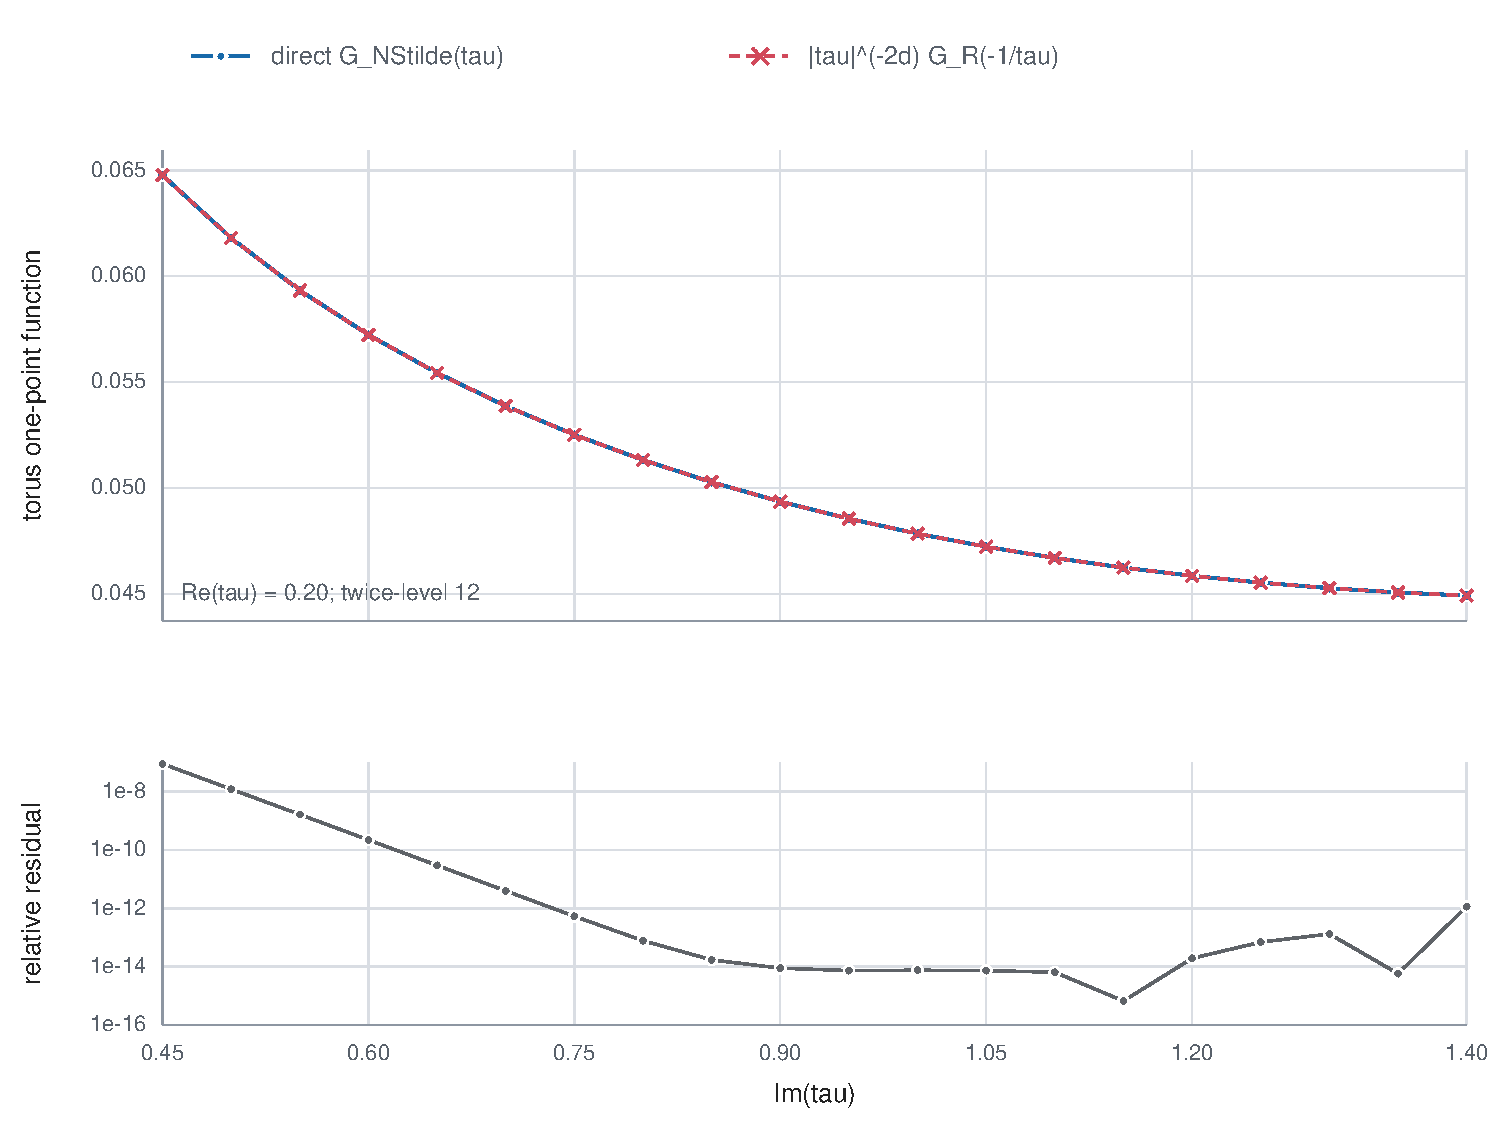
\includegraphics[width=0.96\textwidth]{../../Data Set/results/type0b_torus_modular_cluster/cannon_ns_tilde_r_qscan_20260723_v1/torus_ns_tilde_r_tau_scan.pdf}
 \caption{Two-channel Cannon scan of the
 $\widetilde{\NS}\xleftrightarrow{S}\R$ torus one-point modularity relation
 at $P_{\rm ext}=0.33$, $\operatorname{Re}\tau=0.20$, and maximum
 twice-level $12$.  The upper panel overlays the direct
 $\mathcal G_{\widetilde{\NS}}(\tau)$ evaluation (solid circles) with
 $|\tau|^{-2d}\mathcal G_{\R}(-1/\tau)$ (dashed crosses).  The lower panel
 resolves their relative residual on a logarithmic scale.}
\label{fig:torus-nstilde-r-tau-scan}
\end{figure}

For the accuracy run, the spectral integral is parallelized over
Gauss--Legendre momentum nodes by
\path{super_liouville_torus_modular_cluster.py}.  One worker evaluates the
BRY structure constant and the exact-$c$ finite-part coefficients at one
node, then reuses them for every requested recursion cutoff and modular
frame.  Array tasks write disjoint JSONL shards, and the dependent reduction
job validates the configuration hash, checks that every node occurs exactly
once, sorts by quadrature index, and performs compensated real and imaginary
sums.  Artifact schema 2 additionally requires an exact implementation
fingerprint: SHA-256 hashes of the numerical source closure together with
the Python, NumPy, and \texttt{mpmath} versions are recorded in every shard,
checked before cache reuse and reduction, and copied into the final summary.
Thus the parallel result is deterministic and involves no shared-file
append or silent reuse across code changes.

The default production ledger has 352 node jobs in 16 shards.  It compares
64 and 96 spectral nodes, $P_{\max}=4.5$ and $5.5$, and 32 and 40
finite-part contour samples at 50-decimal structure-constant precision.
For both $\tau=0.2+0.9i$ and the nonprincipal-lift point
$\tau=0.45+0.65i$, it evaluates maximum twice-levels $6,8,10,12$ from the
same prepared coefficients.  A complete eight-process simulation gives
\[
 \delta_{\rm mod}^{\rm principal}=1.55\times10^{-15},\qquad
 \delta_{\rm mod}^{\rm nonprincipal}=1.13\times10^{-10},
\]
while the $64\to96$ quadrature and $P_{\max}:4.5\to5.5$ changes are below
$1.5\times10^{-15}$.  The largest production two-radius diagnostic is
$7.75\times10^{-14}$.  The versioned accuracy configuration and Slurm
launch instructions are in
\path{../../Code/config/type0b_torus_modular_cluster.json} and
\path{cluster/README_type0b_torus_modular.md}.

The Cannon production run, array job \texttt{34584457} followed by reducer
\texttt{34584458}, completed all 352 nodes with zero exit status.  Its
order-12 production values are
\begin{align}
 \mathcal G_{\NS}(0.2+0.9i)
 &=0.05462332460780035,\notag\\
 \mathcal G_{\NS}\!\left(-1/(0.2+0.9i)\right)
 &=0.049916537550511134,
\end{align}
with relative modular residual $1.44329\times10^{-15}$.  At the
nonprincipal-lift point $\tau=0.45+0.65i$, the independently reconstructed
lifts are $(+1,-1)$ and the two frame values are
$0.06179554626182613$ and $0.04761928293035410$, with residual
$1.13284\times10^{-10}$.  The summary and submission record are stored under
\path{../../Data Set/results/type0b_torus_modular_cluster/cannon_q12_20260723_v1/}.  This
historical run predates artifact-schema-2 implementation fingerprinting: its
configuration digest is verified, but the stored numbers are not
cryptographically bound to a source and environment manifest.  A fresh run
with the current driver is required for that stronger certification.

The isolated machine-precision agreement at the first benchmark should not
be mistaken for a generic exact finite-order identity.  Cannon array job
\texttt{34586419} and reducer \texttt{34586420} scan 19 modular parameters.
For the family $\tau=0.2+iy$, the order-12 residual changes as
\[
\begin{array}{c|ccccc}
y&0.45&0.55&0.65&0.75&0.85\\ \hline
\delta_{\rm mod}
&1.98\times10^{-7}&3.00\times10^{-9}&4.66\times10^{-11}
&7.37\times10^{-13}&1.24\times10^{-14}.
\end{array}
\]
With the explicit floor exclusion
$\delta_{\rm mod}>10^{-15}$, seven radial points enter the reproducible
log--log fit
\[
 \delta_{\rm mod}=16.0691\,q_{\max}^{6.461873097\ldots},
 \qquad q_{\max}=\max(|q|,|\widetilde q|).
\]
The fitted exponent is consistent with the expected scaling from the first
omitted NS half-level $q^{6.5}$ after truncation through $q^6$.
The plotting script records the floor, included-point ledger, normalization,
and exponent in \path{torus_modularity_q_scan.fit.json}.
At larger $y$, $|\widetilde q|$ becomes the larger nome and the residual
rises again, producing the modularly symmetric valley in the scan.

The second family, $\tau=0.45+iy$, crosses the transformed-lift boundary
\[
 \operatorname{Re}(-1/\tau)=-\frac12
 \quad\Longleftrightarrow\quad
 y=\sqrt{0.6975}=0.83516\ldots .
\]
The reconstructed lift changes from $(+1,-1)$ to $(+1,+1)$ without any
discontinuity in the correlator or residual.  The 64-to-96 node comparison
changes the assembled correlators by at most $3.19\times10^{-15}$, so the
observed pattern is recursion truncation rather than spectral quadrature.
The historical q-scan reduction gated quadrature and finite-part stability,
but not the modular residual itself.  The current scan configuration adds
order-12 modular-residual gates at the representative principal point
$\tau=0.20+0.85i$ and nonprincipal point $\tau=0.45+0.65i$; these become
certified checks on the next artifact-schema-2 run.

\begin{figure}[!htbp]
 \centering
 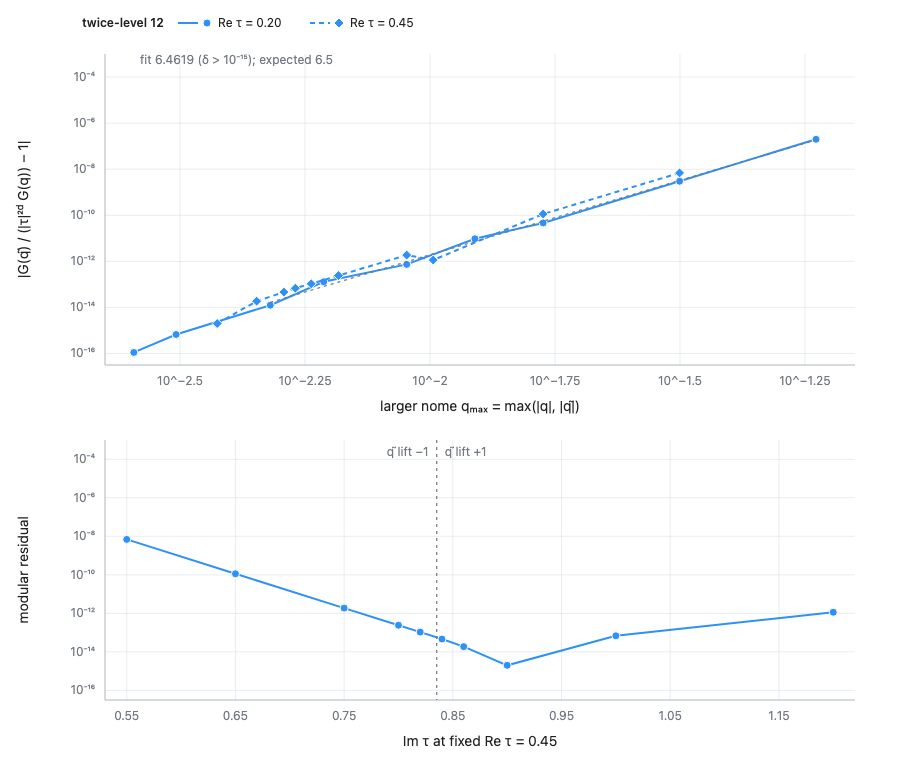
\includegraphics[width=0.92\textwidth]{../../Data Set/results/type0b_torus_modular_cluster/cannon_qscan_20260723_v1/torus_modularity_q_scan.png}
 \caption{Cannon scan of the genus-one NS one-point modular residual at the
 highest recursion cutoff, twice-level $12$.  Solid circles and dashed diamonds are the
 $\operatorname{Re}\tau=0.20$ and $0.45$ families.  The upper panel shows
 the residual against the larger nome; the lower panel resolves the
 transformed NS lift change.}
\label{fig:torus-modularity-q-scan}
\end{figure}

This completes the scalar genus-one one-point function with a bottom NS
external primary in both even-spin modular orbits; it is not yet the entire
physical torus amplitude.  For multipuncture R sewing and higher genus, the
next representation-theory step is to keep the $2\times2$ R ground indices
open at every positive level and recover the scalar
Eq.~\eqref{eq:torus-r-recursion} only after a cycle projection.  The starred
external component, the short quotient at $P=0$, and the Berezin orientation
selecting the physical $G_0$ insertion remain explicit separate tasks.

For the higher-genus $c$-recursion the same operation should be performed
algebraically: store each coefficient as a Laurent/partial-fraction object
in $c$, merge coincident pole keys, and evaluate at $c_0$ only after the
recursive sum is complete.  Equation~\eqref{eq:self-dual-finite-part} is the
sphere implementation and numerical oracle for that graph-level
partial-fraction engine.

\section{Edge-local residue derivation}
\label{sec:residue}

First fix an internal NS edge $e$ of weight $h_e$.  At
$c=c_{rs}(h_e)$, the inverse Gram matrix has a singular rank-one block along
the null submodule.  For descendants $K,L$ above the null state,
\begin{multline}
 \Res_{c=c_{rs}(h_e)}
 (B_{h_e,c}^{(rs/2+n)})^{-1}
 [\mathcal L_K\chi_{rs},\mathcal L_L\chi_{rs}]
 \notag\\
 =J_{rs}(h_e)A_{rs}(h_e)
 (B_{h_e+rs/2,c_{rs}}^{(n)})^{-1}[K,L].
 \label{eq:gram-residue}
\end{multline}
The two vertex tensors adjacent to $e$ factor through
Eqs.~\eqref{eq:null-left}--\eqref{eq:null-right}.  Every other edge and
vertex is a spectator.  Therefore
\begin{equation}
 \Res_{c=c_{rs}(h_e)}\F_{\Gamma}^{\boldsymbol\alpha}
 =q_e^{rs/2}\,\mathcal R_{rs}^{(e)}
 \F_{\Gamma}^{\boldsymbol\alpha}
 \left(c_{rs}(h_e),
       \boldsymbol h+\frac{rs}{2}\ve_e;
       \boldsymbol q\right),
 \label{eq:edge-residue}
\end{equation}
where
\begin{equation}
 \mathcal R_{rs}^{(e)}
 =J_{rs}(h_e)A_{rs}(h_e)
 \Sigma_{rs}^{(v_L,e)}\Sigma_{rs}^{(v_R,e)}.
 \label{eq:edge-r}
\end{equation}
Each $\Sigma$ is the $\sigma$ or $S\sigma$ prescribed by the ordered local
tensor.  Its two weight arguments are the other two legs at that vertex.
For an NS edge this is precisely the CCY locality mechanism with the
replacements
\begin{equation}
 rs\longrightarrow \frac{rs}{2},
 \qquad P_{rs}\longrightarrow\sigma_{rs}^{\alpha},
 \qquad \mathfrak{sl}(2)\longrightarrow\osp.
 \label{eq:replacement-rule}
\end{equation}

Now let $e$ be a generic long Ramond edge and retain its ground indices.
The inverse-Gram residue is a map on the ground fiber and factorizes through
the shifted long module.  Put
\(c_*=c^{\R}_{rs}(\beta_e;\epsilon)\).  Then
\begin{equation}
 \label{eq:r-gram-residue}
\begin{aligned}
 \Res_{c=c_*}
 \left(B_{\R,\beta_e,c}^{(rs/2+n)}\right)^{-1}
 &=J^{\R}_{rs}(\beta_e;\epsilon)A^{\R,(h)}_{rs}\,
 D_{rs}
 \left(B_{\R,\beta'_{rs},c_*}^{(n)}\right)^{-1}
 D_{rs}^{\mathrm{BPZ}},
 \qquad r+s\ \hbox{odd}.
\end{aligned}
\end{equation}
Here the displayed equation is understood as the singular block between
descendants of the two null partners; $D_{rs}$ includes their fixed relative
$G_0$ phase.  Applying the fusion maps at the adjacent vertices gives
\begin{equation}
 \label{eq:r-edge-residue}
\begin{aligned}
 \Res_{c=c_*}
 \mathbf F_{\Gamma}
={}&q_e^{rs/2}J^{\R}_{rs}(\beta_e;\epsilon)
 A^{\R,(h)}_{rs}\,
 \mathbf P_{rs}^{(v_L,e;\epsilon)}
 \mathbf F_{\Gamma}
 \left(c_*,
 \boldsymbol h_{\NS},
 \boldsymbol\beta_{\R}+
 (\beta'_{rs}-\beta_e)\ve_e;\boldsymbol q\right)
 \mathbf P_{rs}^{(v_R,e;\epsilon)}.
\end{aligned}
\end{equation}
The order in Eq.~\eqref{eq:r-edge-residue} is part of the formula.  It
follows the oriented Ramond defect line; exchanging the two matrices can
change the answer.  All nonadjacent graph data are spectators, exactly as in
the NS derivation.

At generic weights the pole positions contributed by different edges are
distinct and all poles are simple.  At coincident or minimal-model values,
the implementation must merge equal pole keys and carry the resulting
higher Laurent orders.  The self-dual finite-part prescription
Eq.~\eqref{eq:self-dual-finite-part} is the tested sphere realization of this
rule.  A one-sided numerical regulator is useful only as an independent
check.

\section{\texorpdfstring{Genus-$g$ NS/R $c$-recursion}
{Genus-g NS/R c-recursion}}
\label{sec:recursion}

Use the mixed analytic coordinates
\begin{equation}
 \mathbf F_\Gamma
 =\mathbf F_\Gamma
 \left(c;\{h_e\}_{e\in E_{\NS}},
          \{\beta_e\}_{e\in E_{\R}};\boldsymbol q\right).
\end{equation}
Thus NS weights and Ramond momenta, rather than Ramond absolute weights, are
held fixed as \(c\) varies.  Assume that the corresponding reduced
plumbing-frame block has a controlled \(c\to\infty\) limit, and keep every
open R ground index.  For each Ramond summand abbreviate
\begin{equation}
\begin{aligned}
 c^*_{e,rs,\epsilon}
 &=c^{\R}_{rs}(\beta_e;\epsilon),
 &\qquad
 \boldsymbol\beta_{\R}^{*}
 &=
 \boldsymbol\beta_{\R}
 +(\beta'_{rs}(b_*)-\beta_e)\ve_e ,
 \\
 \mathcal K^{\R}_{e,rs,\epsilon}(c)
 &=
 \frac{
 q_e^{rs/2}J^{\R}_{rs}(\beta_e;\epsilon)
 A^{\R,(h)}_{rs}(c^*_{e,rs,\epsilon})}
 {c-c^*_{e,rs,\epsilon}} .
\end{aligned}
\end{equation}
The positive-level polar part is
{\small
\begin{align}
 \begin{aligned}
 \mathbf F_{\Gamma}^{\boldsymbol\alpha}
 (c,\boldsymbol h_{\NS},\boldsymbol\beta_{\R};\boldsymbol q)
={}&\mathbf F_{\Gamma,\infty}^{\boldsymbol\alpha}
 (\boldsymbol h_{\NS},\boldsymbol\beta_{\R};\boldsymbol q)
\\
&+\sum_{e\in E_{\NS}}
  \sum_{\substack{r\ge2,\ s\ge1\\r+s\in2\mathbb Z}}
 \frac{q_e^{rs/2}J_{rs}(h_e)A_{rs}(h_e)}
      {c-c_{rs}(h_e)}
 \Sigma_{rs}^{(v_L,e)}\Sigma_{rs}^{(v_R,e)}
 \mathbf F_{\Gamma}^{\boldsymbol\alpha}
 \left(c_{rs}(h_e),
 \boldsymbol h_{\NS}+\frac{rs}{2}\ve_e,
 \boldsymbol\beta_{\R};
 \boldsymbol q\right).
 \end{aligned}
 \label{eq:master-recursion-ns}\\[0.4em]
 \begin{aligned}
 \mathbf F_{\Gamma}^{\boldsymbol\alpha}
 \big|_{\text{R poles}}
={}&
 \sum_{\substack{
 e\in E_{\R},\ r\ge2,\ s\ge1\\
 r+s\in2\mathbb Z+1,\ \epsilon=\pm1}}
 \mathcal K^{\R}_{e,rs,\epsilon}(c)\,
 \mathbf P_{rs}^{(v_L,e;\epsilon)}
 \\
 &\hspace{2.0em}\times
 \mathbf F_{\Gamma}^{\boldsymbol\alpha}
 \left(c^*_{e,rs,\epsilon},
 \boldsymbol h_{\NS},\boldsymbol\beta_{\R}^{*};
 \boldsymbol q\right)
 \mathbf P_{rs}^{(v_R,e;\epsilon)} .
 \end{aligned}
 \label{eq:master-recursion-r}
\end{align}
}
At fixed multi-level $\boldsymbol n$, the sum on edge $e$ is finite:
$rs\le2n_e$.  Hence Eqs.~\eqref{eq:master-recursion-ns} and
\eqref{eq:master-recursion-r} give a triangular coefficient recursion.
The two-dimensional R matrix index is transported through the recursion; it
is not an extra summation over representations.  Choosing a particular R
ground state or GSO component is a boundary contraction performed after the
generic long block has been computed.  Equal \(c_*\) values produced by
different quadratic branches are merged before evaluation.

At fixed \(\beta_e\), the ground denominator is
\begin{equation}
 \frac{1}{h_e^{\R}-c/24}=-\frac{1}{\beta_e^2},
 \label{eq:r-short-c-pole}
\end{equation}
so there is no additional level-zero \(c\)-pole for generic
\(\beta_e\neq0\).  The short module at \(\beta_e=0\) remains a separate
irreducible quotient and is taken only after the generic long block is
constructed.

The formula should be implemented as a recursion on a decorated graph, not
as a new closed expression for each topology.  The topology-dependent data
are only:
\begin{equation}
 (\Gamma,\ s_e,\ \text{half-edge orderings},\ \alpha_v,\ q_e,
 \ \text{spin lift},\ \text{R-defect orientation}).
 \label{eq:graph-data}
\end{equation}
The NS kernel $(c_{rs},J_{rs},A_{rs},\sigma_{rs}^{\alpha})$ and the R kernel
$(c^{\R}_{rs}(\beta;\epsilon),J^{\R}_{rs}(\beta;\epsilon),
A^{\R,(h)}_{rs},\mathbf P_{rs}^{(\epsilon)})$ are universal.

For the theta graph, an NS pole on edge \(e=i\) shifts only \(h_i\), whereas
a Ramond pole shifts only \(\beta_i\to\beta'_{rs}\).  In both cases the
shifted theta block is multiplied by the two fusion factors at the left and
right vertices.  For an NS edge,
\begin{equation}
 \mathcal R_{rs}^{(i)}
 =J_{rs}(h_i)A_{rs}(h_i)
 \Sigma_{rs}^{(L,i)}(h_j,h_k;h_i)
 \Sigma_{rs}^{(R,i)}(h_j,h_k;h_i),
 \qquad\{i,j,k\}=\{1,2,3\}.
 \label{eq:theta-residue}
\end{equation}
The displayed $\Sigma$ notation is intentional: the sign depends on which
slot of each ordered three-point tensor contains edge $i$.  The graph object,
not a handwritten topology formula, is the single source of truth.

\section{\texorpdfstring{The large-$c$ regular part}{The large-c regular part}}
\label{sec:large-c}

\subsection{All-NS super-CCY factorization}

For an all-NS graph, split each descendant into global and non-global modes.
The global
subalgebra is generated by
\begin{equation}
 L_{0,\pm1},\qquad G_{\pm1/2},
 \label{eq:global-algebra}
\end{equation}
and is $\osp$.  The remaining modes are $L_{-n}$ with $n\ge2$ and $G_{-r}$
with $r\ge3/2$.  At fixed weights, Gram--Schmidt can be used to form a basis
whose norms have definite powers of $c$.  Super-Virasoro Ward identities then
force the non-global modes in a leading three-point tensor to contract among
themselves through their central terms.  Dependence on the finite $h_i$ is
subleading in these contractions.  What remains is a product of:
\begin{enumerate}
 \item the same non-global-mode tensor with all modules replaced by the NS
 vacuum module;
 \item a three-point tensor constructed only from $L_{-1}$ and $G_{-1/2}$
 descendants.
\end{enumerate}
The inverse Gram matrices factorize in the same way.  Repeating this at every
vertex yields the super-analogue of the CCY result,
\begin{equation}
 \boxed{
 \F_{\Gamma,\infty}^{\boldsymbol\alpha}
 (\boldsymbol h;\boldsymbol q,\delta)
 =\V_{\Gamma,NS}^{(\infty)}(\boldsymbol q;\delta)
 \ \G_{\Gamma}^{\osp,\boldsymbol\alpha}
 (\boldsymbol h;\boldsymbol q,\delta).}
 \label{eq:large-c-factorization}
\end{equation}
The spin structure $\delta$ enters through the lift of fermionic sewing
around cycles.  Equation~\eqref{eq:large-c-factorization} is the correct seed
organization; it is also the part of the argument that must receive direct
low-level checks at genus two.

The global factor is finite-dimensional representation theory: retain only
$L_{-1}^{n}\nu_h$ and $L_{-1}^{n}G_{-1/2}\nu_h$ on every NS edge and contract
their $\osp$ Gram matrices and vertex tensors on $\Gamma$.  This is a sparse
sum over $(n_e,\beta_e)$ with $\beta_e\in\{0,1\}$.

For a graph with Ramond edges, the polar kernel derived above is unchanged,
but one should not reuse Eq.~\eqref{eq:large-c-factorization} without a
separate large-$c$ analysis.  Integer fermion modes, the $G_0$ ground fiber,
and the Ramond sewing insertion alter the regular seed.  The safe definition
is again direct sewing at large $c$ in the same ordered ground basis.  Thus
the representation-theory residue problem and the R large-$c$ seed problem
are logically separate.

\subsection{Vacuum seed: known checks and the remaining problem}

We define the higher-genus vacuum seed without assuming a closed product:
\begin{equation}
 \V_{\Gamma,NS}^{(\infty)}(\boldsymbol q;\delta)
 \equiv
 \lim_{c\to\infty}
 \F_{\Gamma}^{\mathrm{vac},\delta}(c;\boldsymbol q),
 \label{eq:vacuum-definition}
\end{equation}
where the right-hand side is evaluated by Eq.~\eqref{eq:graph-block} with the
NS vacuum module on every internal and external leg.  This definition fixes
all normalization and signs in the same plumbing frame as the recursion.

At genus one and even NS spin structure it reduces, after removing the
Casimir factor, to the vacuum oscillator character
\begin{equation}
 \V_{1,NS}^{(\infty)}(q)
 =\prod_{n=2}^{\infty}\frac{1+q^{n-1/2}}{1-q^n}.
 \label{eq:torus-vacuum}
\end{equation}
In the bosonic problem, CCY identify the higher-genus vacuum seed, in their
holomorphic plumbing normalization, with
\begin{equation}
 \V_{\Gamma,\mathrm{Vir}}^{(\infty)}
 =\prod_{\gamma\in\mathcal P}\prod_{n=2}^{\infty}
 (1-k_\gamma^n)^{-1/2},
 \label{eq:ccy-schottky}
\end{equation}
where $\mathcal P$ is the set of primitive Schottky conjugacy classes and
$k_\gamma$ is the multiplier.  A supersymmetric analogue should contain a
lift of each Schottky element to the spin bundle, and hence a sign depending
on $\delta$.  We do not assume a particular fermionic product or exponent in
this note.  The safe sequence is:
\begin{equation}
 \begin{aligned}
 \text{direct vacuum sewing}
 &\longrightarrow \text{low-order series in $q_e$}\\
 &\longrightarrow \text{candidate super-Schottky product}\\
 &\longrightarrow \text{coefficient-by-coefficient proof/test}.
 \end{aligned}
 \label{eq:vacuum-sequence}
\end{equation}
This seed, rather than the degenerate pole algebra, is the main unresolved
higher-genus ingredient.

\section{Supergeometry and the sewing ledger}
\label{sec:supergeometry}

The algebraic block does not by itself specify a super-Riemann surface.  For
an NS node, the reduced bosonic sewing parameter is a square of a
superconformal gluing parameter, schematically
\begin{equation}
 q_e=-\varepsilon_e^2.
 \label{eq:ns-plumbing}
\end{equation}
Because NS descendants occur at half-integer level, choosing $q_e$ without a
choice of $\varepsilon_e$ loses the sign of $q_e^{1/2}$.  A numerical block
object must therefore store a lifted parameter or an equivalent spin sign,
not just a complex number $q_e$.  This is also why changing branches inside a
recursion call can spoil crossing or modular covariance.

The dimension of supermoduli space is
\begin{equation}
 \dim\mathfrak M_{g,n_{\NS},n_{\R}}
 =\left(3g-3+n_{\NS}+n_{\R}\ \middle|\
 2g-2+n_{\NS}+\frac{n_{\R}}2\right).
 \label{eq:supermoduli-dimension}
\end{equation}
In particular, a three-NS-punctured sphere has one odd modulus.  The two
kinematic forms $\rho^0$ and $\rho^1$ are the component-level shadow of this
fact.  A physical string amplitude chooses or integrates the corresponding
odd directions through its measure and picture prescription; a chiral block
engine must preserve the label rather than summing it prematurely.

For every plumbing graph we will keep a separate ledger containing:
\begin{equation}
 \boxed{
 \begin{array}{ll}
 \text{edge data:}& \NS/\R,\ h_e,\ q_e,\text{ lift/sign, orientation},\\
 \text{vertex data:}& \text{cyclic half-edge order},\ \alpha_v,
                         \text{odd-modulus convention},\\
 \text{global data:}& \delta,\ \text{homology basis},
                         \text{defect-line routing},\\
 \text{frame data:}& \text{local coordinates and anomaly normalization}.
 \end{array}}
 \label{eq:sewing-ledger}
\end{equation}
The super-Riemann-surface formalism of
Ref.~\cite{Witten2012SuperRiemannSurfaces} supplies these data.  The recursion
kernel consumes them.

\section{Ramond shortening and the geometric sewing boundary}
\label{sec:ramond}

The representation-theory part of a generic long-R edge is now contained in
Eqs.~\eqref{eq:r-ground-action}--\eqref{eq:r-fusion-map}.  No new Kac
mechanism appears at higher genus.  What remains genuinely geometric is the
map that contracts the ground fiber across a Ramond node.

Ramond gluing carries an odd plumbing datum.  In an operator description its
Berezin integral selects a prescribed combination of the identity and $G_0$
on the two-dimensional ground fiber.  That insertion changes the final
ground-index contraction, but not the positive-level pole locations,
null-norm slopes, or fusion polynomials.  It should therefore be represented
as a sewing matrix attached to the edge and applied after
Eq.~\eqref{eq:master-recursion-r}.  Its sign depends on the orientation of the
odd measure.

There are two further boundary choices:
\begin{enumerate}
 \item At $h=c/24$, replace the long module by its irreducible short quotient.
 The normalized two-state basis is singular there, while the unnormalized
 basis \eqref{eq:r-unnormalized-basis} has a regular algebraic limit followed
 by an explicit projection.
 \item In type 0B, the $V^{\R,-}$ family is attached to the fermion-parity
 topological line.  The R ground matrices must be multiplied along an
 oriented defect path or cycle, with junction and GSO phases supplied by the
 sewing ledger.
\end{enumerate}
These choices do not obstruct the generic recursion; they select a component
of the matrix-valued block.  The sphere and torus R recursions fix the local
matrix convention, while the super-Riemann-surface formalism fixes its
higher-genus contraction.

\section{Numerical architecture}
\label{sec:numerics}

The recommended implementation has six layers.
\begin{center}
\begin{tabularx}{\textwidth}{@{}L{0.21\textwidth}X@{}}
\toprule
Layer & Responsibility\\
\midrule
Module algebra & NS bases and the unnormalized long-R ground doublet,
fermionic ordering, Gram matrices, and direct low-level null vectors.\\
Null kernel & Sector-specific Kac labels, branch-tracked $c_{rs}$,
$J_{rs}$, inverse norm slopes $A_{rs}$, and shifted-module parameters.\\
Vertex kernel & NS fusion scalars $\sigma_{rs}^{0,1}$, R fusion matrices
$\mathbf P_{rs}$, Ward-identity phases, and canonical slot orderings.\\
Meromorphic ledger & Laurent/partial-fraction coefficients in $c$, merged
coincident pole keys, higher pole orders, and finite-part evaluation only
after a complete recursive coefficient has been assembled.\\
Decorated graph & Topology, half-edge order, component labels, edge sectors,
plumbing lifts, R-defect orientation, and sparse multi-level truncation.\\
Seed and recursion & Sector-appropriate large-$c$ seed, memoized edge-local
recursion, ground-index contractions, and numerical error ledger.\\
\bottomrule
\end{tabularx}
\end{center}

A coefficient evaluator at total twice-level cutoff $L$ should:
\begin{enumerate}
 \item enumerate multi-levels $\ell_e=2n_e\in\mathbb Z_{\ge0}$ with
 $\sum_e\ell_e\le L$;
 \item evaluate the large-$c$ seed coefficient;
 \item for each NS edge enumerate $r+s$ even and for each R edge enumerate
 $r+s$ odd, always with $r\ge2$, $s\ge1$, and $rs\le\ell_e$;
 \item multiply $J_{rs}A_{rs}$ by the two canonicalized NS fusion scalars or
 by the ordered pair of R fusion matrices;
 \item recurse at the sector-specific $c_{rs}(h_e)$ with
 $h_e\mapsto h_e+rs/2$ and
 $\ell_e\mapsto\ell_e-rs$;
 \item memoize by the full shifted weight tuple, central charge, multi-level,
 component tuple, R ground indices, and branch/lift identifiers.
\end{enumerate}
Memoizing only numerical $q_e$ and weights is insufficient because two spin
lifts can have the same reduced $q_e$.

\section{Validation ladder}
\label{sec:tests}

The implementation should not begin with a physical genus-two integral.  The
following ladder isolates errors cheaply.
\begin{enumerate}
 \item \textbf{Algebra.} Reproduce
 $\langle G_{-1/2}\nu_h|G_{-1/2}\nu_h\rangle=2h$ and the direct Gram and
 three-point tensors through at least total level $2$.  In the R module verify
 $G_0^2=h-c/24$, $\det B_{\R}^{(0)}=h-c/24$, and the level-one Kac zero.
 \item \textbf{NS sphere.} Recover every coefficient produced by the existing
 \texttt{superconformal\_blocks.py} layer, including starred external components and
 the $S_{rs}^{\alpha}$ sign.
 \item \textbf{Four-R sphere.} With NS exchange, reproduce
 Eqs.~\eqref{eq:four-r-elliptic-recursion}--\eqref{eq:four-r-direct-anchors}
 for all four HJS chiral sign branches.  This calibrates
 $P_{\NS|\R\R}^{rs}$ and the odd--odd phase, but not an R internal edge.
 \item \textbf{R-internal sphere.} At generic complex $\beta$, use a
 two-NS/two-R ordering with R exchange to reproduce the two
 $\pm\beta_{rs}$ residues and verify that converting them to a weight pole
 gives Eqs.~\eqref{eq:r-a-weight}--\eqref{eq:r-a-beta}.  Reproduce the direct
 descendant coefficients through at least $q^3$, as in
 Sec.~\ref{sec:r-bruteforce-q3}, and keep all ground indices open before any
 nonchiral contraction.
 \item \textbf{Torus.} Recover Eq.~\eqref{eq:torus-vacuum}, the published NS
 one-point recursions, and the generic long-R toric recursion including the
 shift $\beta_{rs}\mapsto\beta'_{rs}$.
 \item \textbf{Residue.} For a generic complex weight, compare a numerical
 finite-difference residue of direct sewing with
 Eqs.~\eqref{eq:edge-residue}, \eqref{eq:edge-r}, and
 \eqref{eq:r-edge-residue}.
 \item \textbf{All-NS genus two.} Compare recursion and direct theta-graph sewing
 coefficient by coefficient at total twice-level $L=2,4,6$ before increasing
 the cutoff.
 \item \textbf{Mixed genus.} Choose the smallest graph containing an oriented
 R cycle, keep its ground indices open, and compare direct sewing with the
 ordered matrix recursion before applying the odd-plumbing or GSO projector.
 \item \textbf{Geometry.} Flip one plumbing lift while holding $q_e$ fixed
 and verify the predicted sign of half-integer-level terms.  Then check graph
 automorphisms and a basic change of pants channel.
 \item \textbf{Shortening.} Approach $\beta=0$ in the unnormalized basis,
 project out $G_0w^+$, and compare with a direct short-module computation.
 \item \textbf{Seed.} Only after the direct vacuum coefficients are stable,
 test a proposed super-Schottky primitive-class product.
\end{enumerate}

For the type-0B application, generic complex $c$ remains useful while
debugging individual residues and branches.  Production coefficients at
$c=27/2$ should instead be assembled as Laurent/partial-fraction objects and
evaluated only after coincident poles have been merged.  On the sphere,
Eq.~\eqref{eq:self-dual-finite-part} implements this rule directly; the old
$c_0\pm\epsilon$ average is retained as an independent regression.

\section{Status and immediate next calculation}

\begin{center}
\begin{tabularx}{\textwidth}{@{}L{0.30\textwidth}L{0.18\textwidth}X@{}}
\toprule
Ingredient & Status & Next action\\
\midrule
Ordinary-$c$ NS pole locations and Jacobian & Fixed & Reuse the tested sphere
kernel.\\
RRRR/NSNSRR fixed-weight \(c\)-pole experiment & Retained as a local
residue test only & First \((3,1)\) and \((2,2)\) residues agree with the
independent \(h\)-recursion.  Replace its analytic slice by fixed Ramond
\(\beta_i\); do not reuse its fixed-\(h_i^{\R}\) large-\(c\) seed.\\
NS null norm and two fusion families & Fixed & Refactor into a topology-free
module with canonical orientations.\\
Four-R sphere block with NS exchange & Implemented and tested & Reuse the
fixed HJS-to-BRY sign map in later nonchiral contractions.\\
Exact $b=1$ collision handling & Implemented for sphere coefficients &
Promote the tested finite-part oracle to graph-level partial fractions in
$c$.\\
RRRR physical crossing & Implemented and tested & Retain as a regression for
the HJS-to-BRY chiral sign dictionary.\\
Generic long-R sphere block & Implemented and tested & Level-one direct
sewing, direct descendants through $q^3$, exact-$c$ finite part, and RRNSNS
mixed-sector crossing pass.\\
NS/R torus one-point kernel & Exact $b=1$, $2n_{\max}=12$;
$S$ error $1.6\times10^{-15}$ & Open the positive-level R ground indices before the
cycle projection; then test the $\widetilde{\NS}\leftrightarrow\R$ orbit.\\
NS torus two-point necklace & Two-edge h-recursion and
$dP_a\,dP_b/\pi^2$ assembly implemented & Extend the direct Ward/Gram oracle
beyond level one and run production four-parameter convergence scans.\\
R-handle NS two-point necklace & Paired beta-pole recursion, all sign/cycle
sectors, exact-$b=1$ finite part, and spectral assembly through level one &
Derive the contracted all-level R regular seed and replace the direct
Ward/Gram seed oracle.\\
R null norm and fusion matrices & Sphere scalar components calibrated & Lift
the tested local residue to open ground-fiber matrices for graph sewing.\\
Arbitrary-graph NS/R polar recursion & Derived & Implement sector-decorated
edges and ordered matrix insertions.\\
$\osp$ global factor & Fixed in principle & Implement sparse global-mode
contractions for the all-NS graph.\\
Higher-genus NS vacuum seed & Open but sharply defined & Compute the theta
vacuum series directly through low total level; only then identify a closed
Schottky formula.\\
R large-$c$ seed and odd sewing matrix & Open but separated & Obtain by
direct long-R sewing in a fixed Berezin convention.\\
Spin structure and defect routing & Ledger specified & Fix one genus-two
homology, plumbing, and oriented R-cycle convention.\\
Short R ground state & Boundary case isolated & Project the unnormalized
long module at $\beta=0$ after generic tests pass.\\
\bottomrule
\end{tabularx}
\end{center}

The sphere calibration now includes four-R/NS exchange through order $12$ at
the exact self-dual point, the generic long-R direct Gram/Ward calculation
through $q^3$, and physical RRRR and RRNSNS crossing.  The genus-one layer
adds the NS spin lift, both scalar HJS R projections, and an explicit
$G_0$ ground-fiber closure.  The local $G_0$ action and scalar R residue are
therefore fixed through three descendant levels.  The next calculation is
to keep both Ramond ground indices open at every positive level and promote
the tested scalar factors to the ordered matrices
$J^{\R}_{rs}(\beta;\epsilon)A^{\R,(h)}_{rs}
\mathbf P_L^{(\epsilon)}\mathbf P_R^{(\epsilon)}$.  Every component should
first be matched to direct two-NS/two-R sewing and to the published toric
block.  This matching and the subsequent large-\(c\) analysis must keep
every Ramond \(\beta\) fixed.  Only then should the matrix be inserted on an
oriented R cycle of a genus-two graph.  In parallel, the all-NS theta block
at total twice-level
$L=2$ and $4$ should be compared between direct sewing and
Eq.~\eqref{eq:master-recursion-ns}, with coincident $c$ poles stored in a
merged partial-fraction ledger.  These tests separate the remaining
ground-fiber routing and orientation choices from the higher-genus seed and
sewing ledger.

\section{Conclusion}

The CCY locality argument extends to both NS and generic long-R
super-Virasoro modules.  In either sector the polar coefficient is exactly
$J_{rs}A_{rs}$ times one null-vector fusion factor at each endpoint.  The R
sector replaces scalar endpoint data by ordered maps on a two-dimensional
$G_0$ ground fiber; the fiber dimension is unchanged by the null-module
shift.  Its natural \(c\)-plane coordinate keeps \(\beta\), rather than
\(h_{\R}\), fixed.  Hence the genus-$g$ polar recursion is not a new representation
problem: it is graph assembly of the sphere-tested local kernel.

The genuinely new higher-genus work lies in the regular large-$c$ seed and
in the supergeometric contraction data.  Spin lifts, odd Ramond plumbing, and
defect routing select components of the algebraic matrix block but do not
modify its positive-level Kac residues.  The short R ground state is a
controlled quotient at $\beta=0$, not a new generic recursion.  This
separation gives a precise route from known four-point representation theory
to a numerical genus-$g$ block engine.

\clearpage
\bibliographystyle{unsrt}
\bibliography{../../References/references}

\end{document}
